\documentclass[12pt]{report}

\usepackage[english]{babel}
\usepackage[T1]{fontenc}
\usepackage[utf8]{inputenc}
\usepackage{titlesec}
\usepackage{setspace}
\usepackage{graphicx}
\usepackage[hidelinks]{hyperref}
\usepackage{array}
\usepackage{times}
\usepackage{upgreek}
\usepackage{todonotes}
\usepackage{url}
\usepackage{longtable}
\usepackage{pdflscape}
\usepackage{booktabs}
\usepackage{amsmath}
\usepackage{amssymb}

\graphicspath{{assets/}}
\renewcommand{\contentsname}{Table of Contents}
\doublespacing

\title{A Comparative Analysis on Feature Selection for Regression Models: Comparing SHAP-Based Methods with Traditional Approaches}
\author{Artur Temporal Coelho}
\date{2026}

\begin{document}

\begin{titlepage}
    \begin{center}
        \vspace*{1cm}

        \Huge
        \textbf{A Comparative Analysis on Feature Selection for Regression Models: Comparing SHAP-Based Methods with Traditional Approaches}\\

        \vspace{0.5cm}

        \LARGE
        Master's Thesis

        \vspace{3cm}

        \textbf{Student:}\\
        Artur Temporal Coelho\\

        \vspace{0.5cm}

        \textbf{Supervisor:}\\
        Jesús Javier Rodríguez Sala\\

        \vspace{1cm}

        \textbf{Institution:}\\
        Universidad Miguel Hernandez\\

        \vspace{0.5cm}

        \textbf{Program:}\\
        Máster Universitario en Estadística Computacional y Ciencia de Datos para la Toma de Decisiones

        \vfill

        \Large
        2026

    \end{center}
\end{titlepage}

\pagenumbering{roman}

\begin{center}
\LARGE
\textbf{Acknowledgements}
\end{center}


\newpage

\begin{center}
\LARGE
\textbf{Abstract}
\end{center}

This thesis evaluates SHAP-based feature selection for tabular regression against established methods including mutual information, recursive feature elimination, and tree-based importance. The study uses a two-stage protocol: broad screening across four datasets and three model families, followed by focused evaluation with custom SHAP recursive elimination and hybrid strategies.

Results show that SHAP-based selection achieves competitive but not superior performance. In the broad benchmark, SHAP wins in only 2 of 12 dataset-model configurations. Hybrid strategies add complexity without corresponding accuracy gains.

The conclusion is that SHAP remains primarily valuable for model explanation rather than feature selection. Under computational constraints, simpler methods such as mutual information remain the pragmatic default.

\vspace{0.5cm}

\textbf{Keywords:} feature selection, SHAP, regression, machine learning, model interpretability, TreeExplainer.

\newpage

\tableofcontents
\newpage

\listoffigures
\listoftables
\newpage

\pagenumbering{arabic}

\chapter{Introduction}

Machine learning has transformed how organizations extract value from data, enabling predictive models that automate decisions in domains ranging from financial risk assessment to industrial process optimization. Among the many tasks addressed by machine learning, regression (the prediction of continuous outcomes) remains fundamental. Whether estimating insurance claim costs, forecasting energy demand, or predicting material properties, regression models serve as the backbone of quantitative decision support systems.

As datasets grow in both volume and dimensionality, practitioners face an increasingly common challenge: determining which input variables actually contribute to accurate predictions. High-dimensional datasets may contain hundreds or thousands of features, yet only a subset typically carries meaningful predictive signal. The remaining features introduce noise, increase computational burden, and complicate model interpretation. Feature selection addresses this challenge by identifying and retaining only the most informative variables before or during model training.

\section{Context and Motivation}

The importance of feature selection extends beyond dimensionality reduction. Effective selection can improve generalization by reducing overfitting, decrease training and inference time, lower storage, and when applied with model explanation strategies, produce models that are easier to explain and maintain. In regulated industries or high-stakes applications, the ability to articulate why a model uses specific inputs is often as important as the accuracy of its predictions.

Traditional feature selection methods fall into three categories: filter methods that rank features by statistical criteria independently of the model, wrapper methods that evaluate subsets through iterative model training, and embedded methods where selection occurs as part of the learning algorithm itself~\cite{guyon2003introduction}. Each approach involves trade-offs between computational cost, model dependency, and theoretical guarantees.

Model interpretability tools have gained prominence, with SHAP (SHapley Additive exPlanations) emerging as a influential framework~\cite{lundberg2020local}. SHAP provides theoretically grounded feature attributions derived from cooperative game theory~\cite{shapley1953value}, offering both local explanations for individual predictions and global importance rankings across datasets~\cite{fryer2021shapley}. While SHAP is primarily designed for explanation, its global importance scores can be repurposed for feature selection. This raises a question: does SHAP-based selection offer advantages over established methods, or does its explanatory elegance come without corresponding gains in predictive utility?

\section{Problem Statement}

Despite SHAP's widespread adoption for model interpretation, its effectiveness as a feature selection mechanism remains underexplored in systematic comparisons. Some recent work has questioned whether SHAP importance rankings translate reliably into effective feature subsets~\cite{wang2024feature}, while others have reported promising results~\cite{marcilio2020explanations}. Existing literature often showcases SHAP in explanatory contexts without rigorous benchmarking against traditional selectors across diverse datasets and model families. Furthermore, SHAP computation, even with efficient implementations like TreeExplainer~\cite{lundberg2020local}, incurs non-trivial runtime costs that may not be justified if simpler methods achieve comparable results.

This gap creates uncertainty for practitioners who must choose feature selection strategies under real-world constraints. Without clear evidence on when SHAP-based selection provides meaningful benefits, organizations risk either underutilizing a powerful tool or investing computational resources in approaches that offer little marginal advantage.

\section{Objectives}

\subsection{General Objective}

This thesis aims to evaluate SHAP-based feature selection for tabular regression problems, comparing its predictive effectiveness, computational cost, and selection stability against established alternatives across multiple datasets and model families.

\subsection{Specific Objectives}

\begin{enumerate}
    \item Conduct a broad benchmark comparing mutual information, recursive feature elimination, tree-based importance, and SHAP-based selection across four datasets and three model types.
    \item Quantify the trade-offs between prediction error reduction and execution time for each strategy under varying feature retention levels.
    \item Measure selection stability, meaning the consistency of chosen feature subsets across repeated experimental runs, to assess method robustness.
    \item Perform a focused evaluation using the best-performing model from the broad benchmark, testing custom SHAP recursive elimination and hybrid strategies.
    \item Synthesize practical recommendations for choosing feature selection methods in applied regression projects.
\end{enumerate}

\section{Scope and Limitations}

This work is positioned as an applied master's thesis: the goal is not to propose novel algorithms, but to produce a structured, reproducible comparison that yields actionable guidance. The study is limited to supervised tabular regression, four datasets in the broad screening stage, two datasets in the deep-dive stage, and the specific model families and selection strategies implemented in the experimental pipeline.

The analysis does not claim exhaustive coverage of all explainability approaches, all regression estimators, or all hyperparameter optimization schemes. Results should be interpreted as context-sensitive empirical findings applicable to similar tabular regression settings, rather than universal claims. Detailed references are deferred to a subsequent revision pass.

\section{Document Structure}

The remainder of this thesis is organized as follows. Chapter~2 reviews the current state of regression modeling, feature selection techniques, and SHAP methodology, establishing the technical foundation for the experiments. Chapter~3 formalizes the research hypotheses and describes the experimental design, including the two-stage approach with broad screening followed by focused evaluation. Chapter~4 presents the methodology in detail and reports the experimental results, with emphasis on performance, stability, and cost trade-offs. Chapter~5 concludes with a synthesis of findings, practical recommendations, and directions for future work.

\chapter{State of the Art}

This chapter reviews the technical foundations underlying this thesis: regression modeling approaches for tabular data, feature selection methodologies, and the SHAP framework with particular attention to TreeExplainer. The review establishes both the theoretical background and practical considerations that inform the experimental design.

\section{Regression Modeling for Tabular Data}

Tabular data, structured records with rows representing observations and columns representing features, remains the dominant format in business and scientific applications. Unlike images or text, tabular datasets present heterogeneous feature types, varying scales, and often complex correlation structures that require careful modeling choices.

\subsection{Linear Models}

Regularized linear regression, particularly Ridge regression~\cite{hoerl1970ridge}, provides a baseline approach with well-understood properties. Ridge regression minimizes the sum of squared residuals plus an L2 penalty on coefficient magnitudes:

\begin{equation}
\hat{\beta} = \arg\min_{\beta} \left( \|y - X\beta\|^2 + \lambda\|\beta\|^2 \right)
\end{equation}

This formulation shrinks coefficients toward zero without eliminating them entirely, providing some implicit feature weighting. Linear models are computationally efficient and interpretable, but may underperform when relationships between features and target are nonlinear.

\subsection{Ensemble Tree Methods}

Tree-based ensembles have become the dominant approach for tabular regression~\cite{breiman2001random}. Two architectures are particularly relevant:

\textbf{Bagging ensembles}, exemplified by ExtraTrees (Extremely Randomized Trees)~\cite{geurts2006extremely}, construct multiple decision trees on bootstrap samples with additional randomization in split selection. By averaging predictions across trees, these methods reduce variance while maintaining the ability to capture nonlinear relationships and feature interactions.

\textbf{Gradient boosting}, exemplified by XGBoost~\cite{chen2016xgboost}, builds trees sequentially where each tree corrects the residual errors of its predecessors. This additive training approach often achieves state-of-the-art performance on structured data, though it introduces more hyperparameters and potential for overfitting compared to bagging methods.

Both ensemble types provide native feature importance measures: for bagging ensembles, importance typically reflects how often a feature is used in splits weighted by the improvement achieved; for gradient boosting, importance can be measured by gain (total reduction in loss from splits using that feature), weight (split frequency), or cover (number of samples affected).

\section{Feature Selection Strategies}

Feature selection methods are conventionally categorized into three families based on their relationship with the learning algorithm~\cite{guyon2003introduction}.

\subsection{Filter Methods}

Filter methods evaluate features independently of any specific model, typically using statistical measures of relevance. Mutual Information (MI) is a widely used filter criterion that captures arbitrary dependencies between a feature $X$ and target $Y$:

\begin{equation}
MI(X; Y) = \sum_{x,y} p(x,y) \log \frac{p(x,y)}{p(x)p(y)}
\end{equation}

For continuous variables, MI is estimated through discretization or kernel density methods. Filter methods are computationally cheap and model-agnostic, but ignore feature interactions and may select redundant variables.

\subsection{Wrapper Methods}

Wrapper methods evaluate feature subsets by training the target model and measuring performance. Recursive Feature Elimination (RFE) is a prominent example: starting with all features, RFE iteratively removes the least important feature(s) according to the model's own importance scores, continuing until a desired subset size is reached. While wrapper methods account for model-specific behavior, they are computationally expensive and may overfit to the evaluation metric.

\subsection{Embedded Methods}

Embedded methods perform selection as part of model training. L1-regularized regression (Lasso)~\cite{tibshirani1996lasso} is the canonical example, where the penalty term drives some coefficients exactly to zero. Tree-based models also embed implicit selection by only splitting on informative features. This thesis treats tree-based native importance as an embedded approach, though it can also serve as input to explicit subset selection.

\section{SHAP: Theory and Computation}

SHAP (SHapley Additive exPlanations)~\cite{lundberg2017unified} provides a unified framework for feature attribution that satisfies desirable theoretical properties from cooperative game theory. Understanding SHAP requires examining both its theoretical foundations and practical computational approaches.

\subsection{Shapley Values in Feature Attribution}

The core idea borrows from cooperative game theory, where Shapley values~\cite{shapley1953value} fairly distribute a total payoff among players according to their marginal contributions. In the feature attribution context, features are ``players'' and the ``payoff'' is the model prediction minus a baseline (typically the expected prediction).

For a model $f$, the Shapley value $\phi_j$ for feature $j$ is defined as:

\begin{equation}
\phi_j = \sum_{S \subseteq N \setminus \{j\}} \frac{|S|!(|N|-|S|-1)!}{|N|!} \left[ f(S \cup \{j\}) - f(S) \right]
\end{equation}

where $N$ is the set of all features, $S$ is a subset excluding feature $j$, and $f(S)$ represents the model prediction when only features in $S$ are ``present'' (with absent features marginalized out). This formula averages the marginal contribution of feature $j$ over all possible orderings in which features could be added.

Shapley values uniquely satisfy four axioms~\cite{fryer2021shapley}:
\begin{itemize}
    \item \textbf{Efficiency}: attributions sum to the difference between the prediction and baseline.
    \item \textbf{Symmetry}: features with identical contributions receive identical attributions.
    \item \textbf{Dummy}: features that never change predictions receive zero attribution.
    \item \textbf{Linearity}: attributions combine linearly across additive models.
\end{itemize}

For feature selection, global importance is typically computed by averaging absolute SHAP values across all observations: $I_j = \frac{1}{n}\sum_{i=1}^{n}|\phi_j^{(i)}|$.

\subsection{TreeExplainer: Efficient SHAP for Tree Ensembles}

The na\"ive computation of Shapley values requires evaluating exponentially many feature subsets, which is intractable for high-dimensional data. TreeExplainer~\cite{lundberg2020local} exploits the structure of decision trees to compute exact SHAP values in polynomial time.

The key insight is that a decision tree already partitions the feature space into regions, and the path from root to leaf for any observation defines which features were used. TreeExplainer recursively propagates SHAP values through the tree structure, correctly handling the exponential number of coalitions by clever bookkeeping of how predictions change as features are revealed or hidden.

For an ensemble of $T$ trees, each with $L$ leaves and average depth $D$, TreeExplainer computes exact SHAP values in $O(TLD^2)$ time per observation. Here, $T$ is the number of trees in the ensemble, $L$ is the number of leaves per tree, and $D$ is the tree depth. This is dramatically faster than model-agnostic approaches but still represents non-trivial overhead compared to simply extracting native importance scores.

\subsection{Practical Considerations}

Several factors affect SHAP computation in practice:

\textbf{Sample size}: computing SHAP for all training observations may be expensive; practitioners often use a representative sample.

\textbf{Background data}: SHAP values depend on a reference distribution used to marginalize absent features. TreeExplainer typically uses the training data itself as background.

\textbf{Stability}: because tree ensembles are stochastic (due to random splits or bootstrap sampling), SHAP rankings may vary between model fits, potentially affecting selection consistency.

\section{Datasets for Evaluation}

Before running long experiments, a pre-study pipeline was executed to download, preprocess, and characterize each dataset. This section summarizes the four datasets selected for the broad benchmark, chosen to span different scales and correlation structures.

\begin{table}[h]
\centering
\caption{Dataset characteristics after preprocessing.}
\label{tab:datasets}
\begin{tabular}{lrrrrl}
\toprule
\textbf{Dataset} & \textbf{Rows} & \textbf{Num.} & \textbf{Cat.} & \textbf{Target} & \textbf{Domain} \\
\midrule
Allstate Claims~\cite{gaurallstate} & 188,318 & 14 & 116 & loss & Insurance \\
Bike Sharing~\cite{fanaee2014event} & 17,379 & 12 & 0 & cnt & Rentals \\
Communities \& Crime~\cite{redmond2002data} & 1,993 & 100 & 0 & ViolentCrimesPerPop & Crime \\
Superconductor~\cite{hamidieh2018superconductor} & 21,263 & 81 & 0 & critical\_temp & Materials \\
\bottomrule
\end{tabular}
\end{table}

This collection provides diversity along several axes:

\textbf{Scale}: from under 2,000 observations (Communities and Crime) to nearly 200,000 (Allstate), testing whether method behavior differs with sample size.

\textbf{Dimensionality}: from 12 features (Bike Sharing) to 130 features (Allstate), covering both low and high-dimensional regimes.

\textbf{Correlation structure}: the pre-study correlation heatmaps reveal that some datasets exhibit strong feature clusters (Communities and Crime) while others show more dispersed correlation patterns.

\begin{figure}[p]
    \centering
    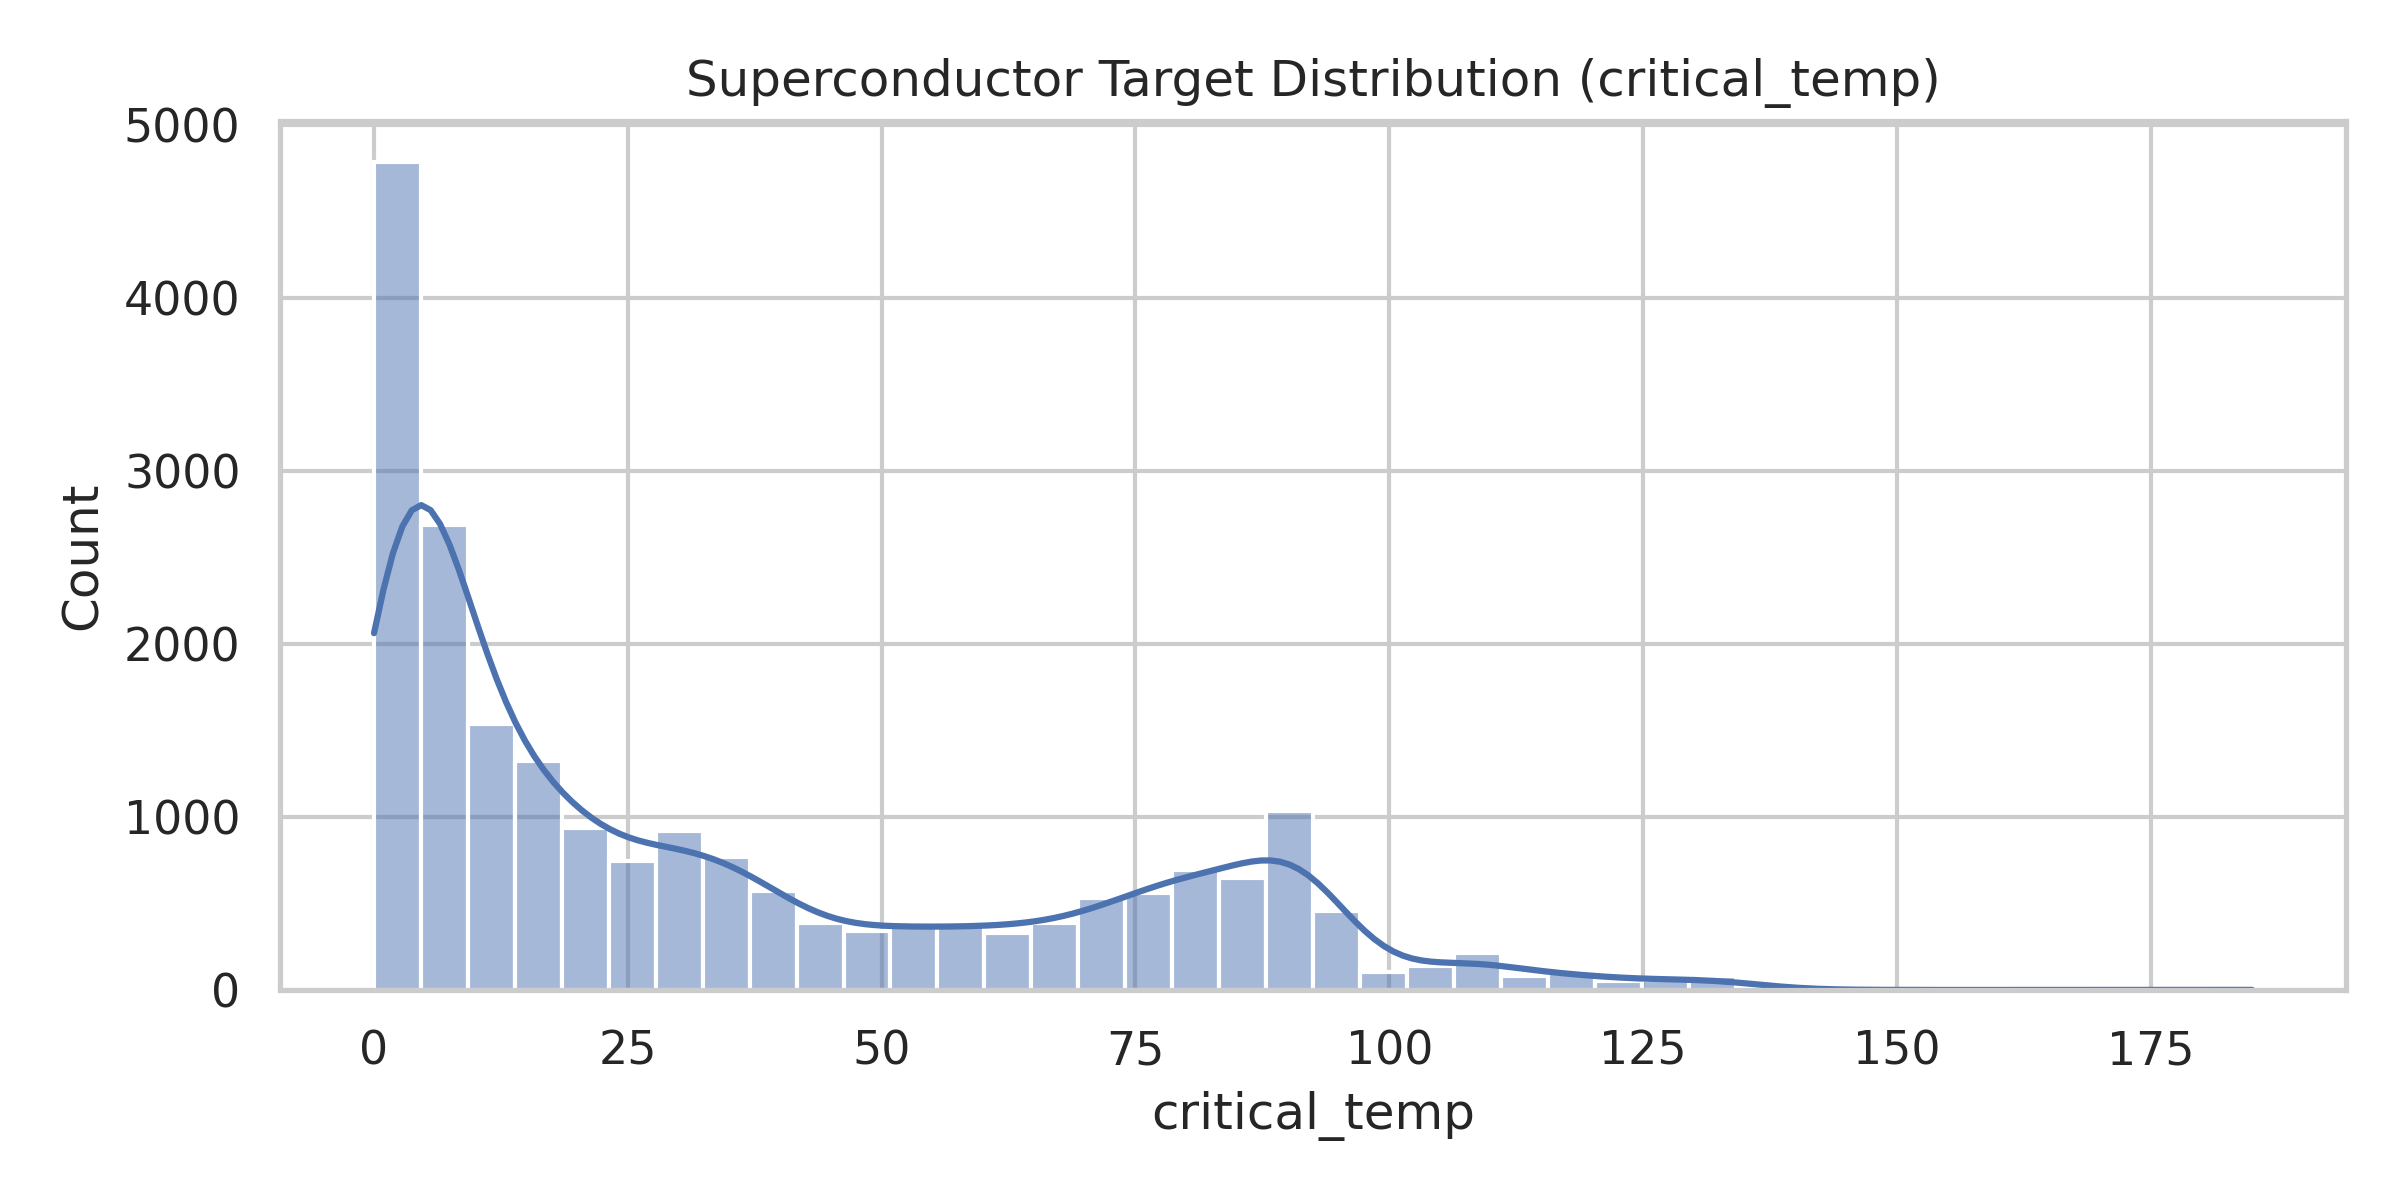
\includegraphics[width=0.65\textwidth]{../pre_study/figures/superconductor_target_distribution.png}\\[0.3em]
    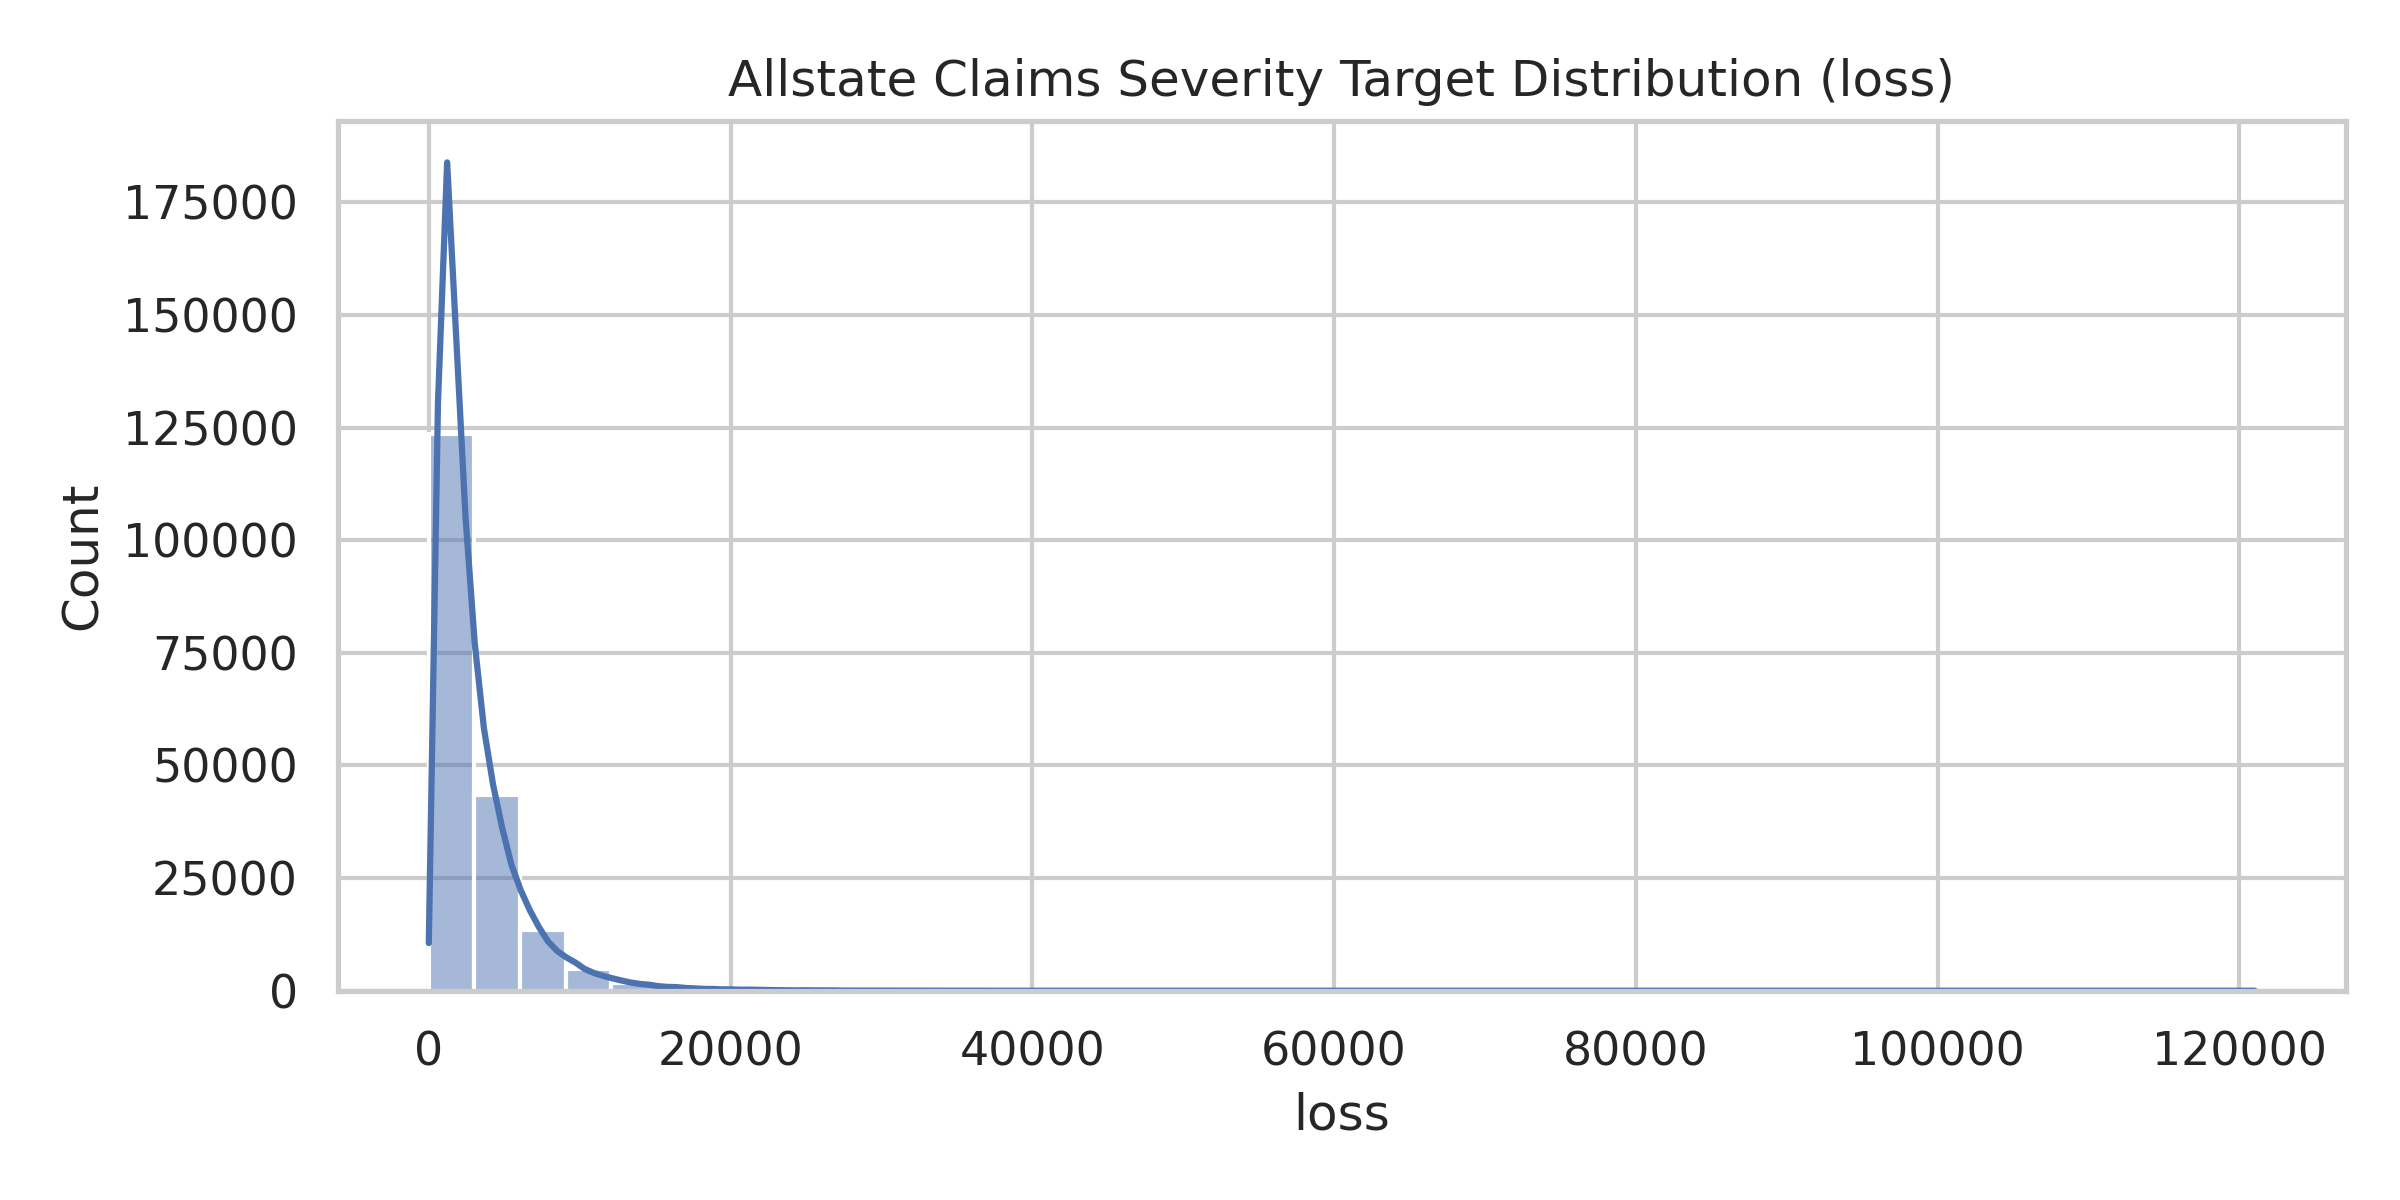
\includegraphics[width=0.65\textwidth]{../pre_study/figures/allstate_claims_target_distribution.png}\\[0.3em]
    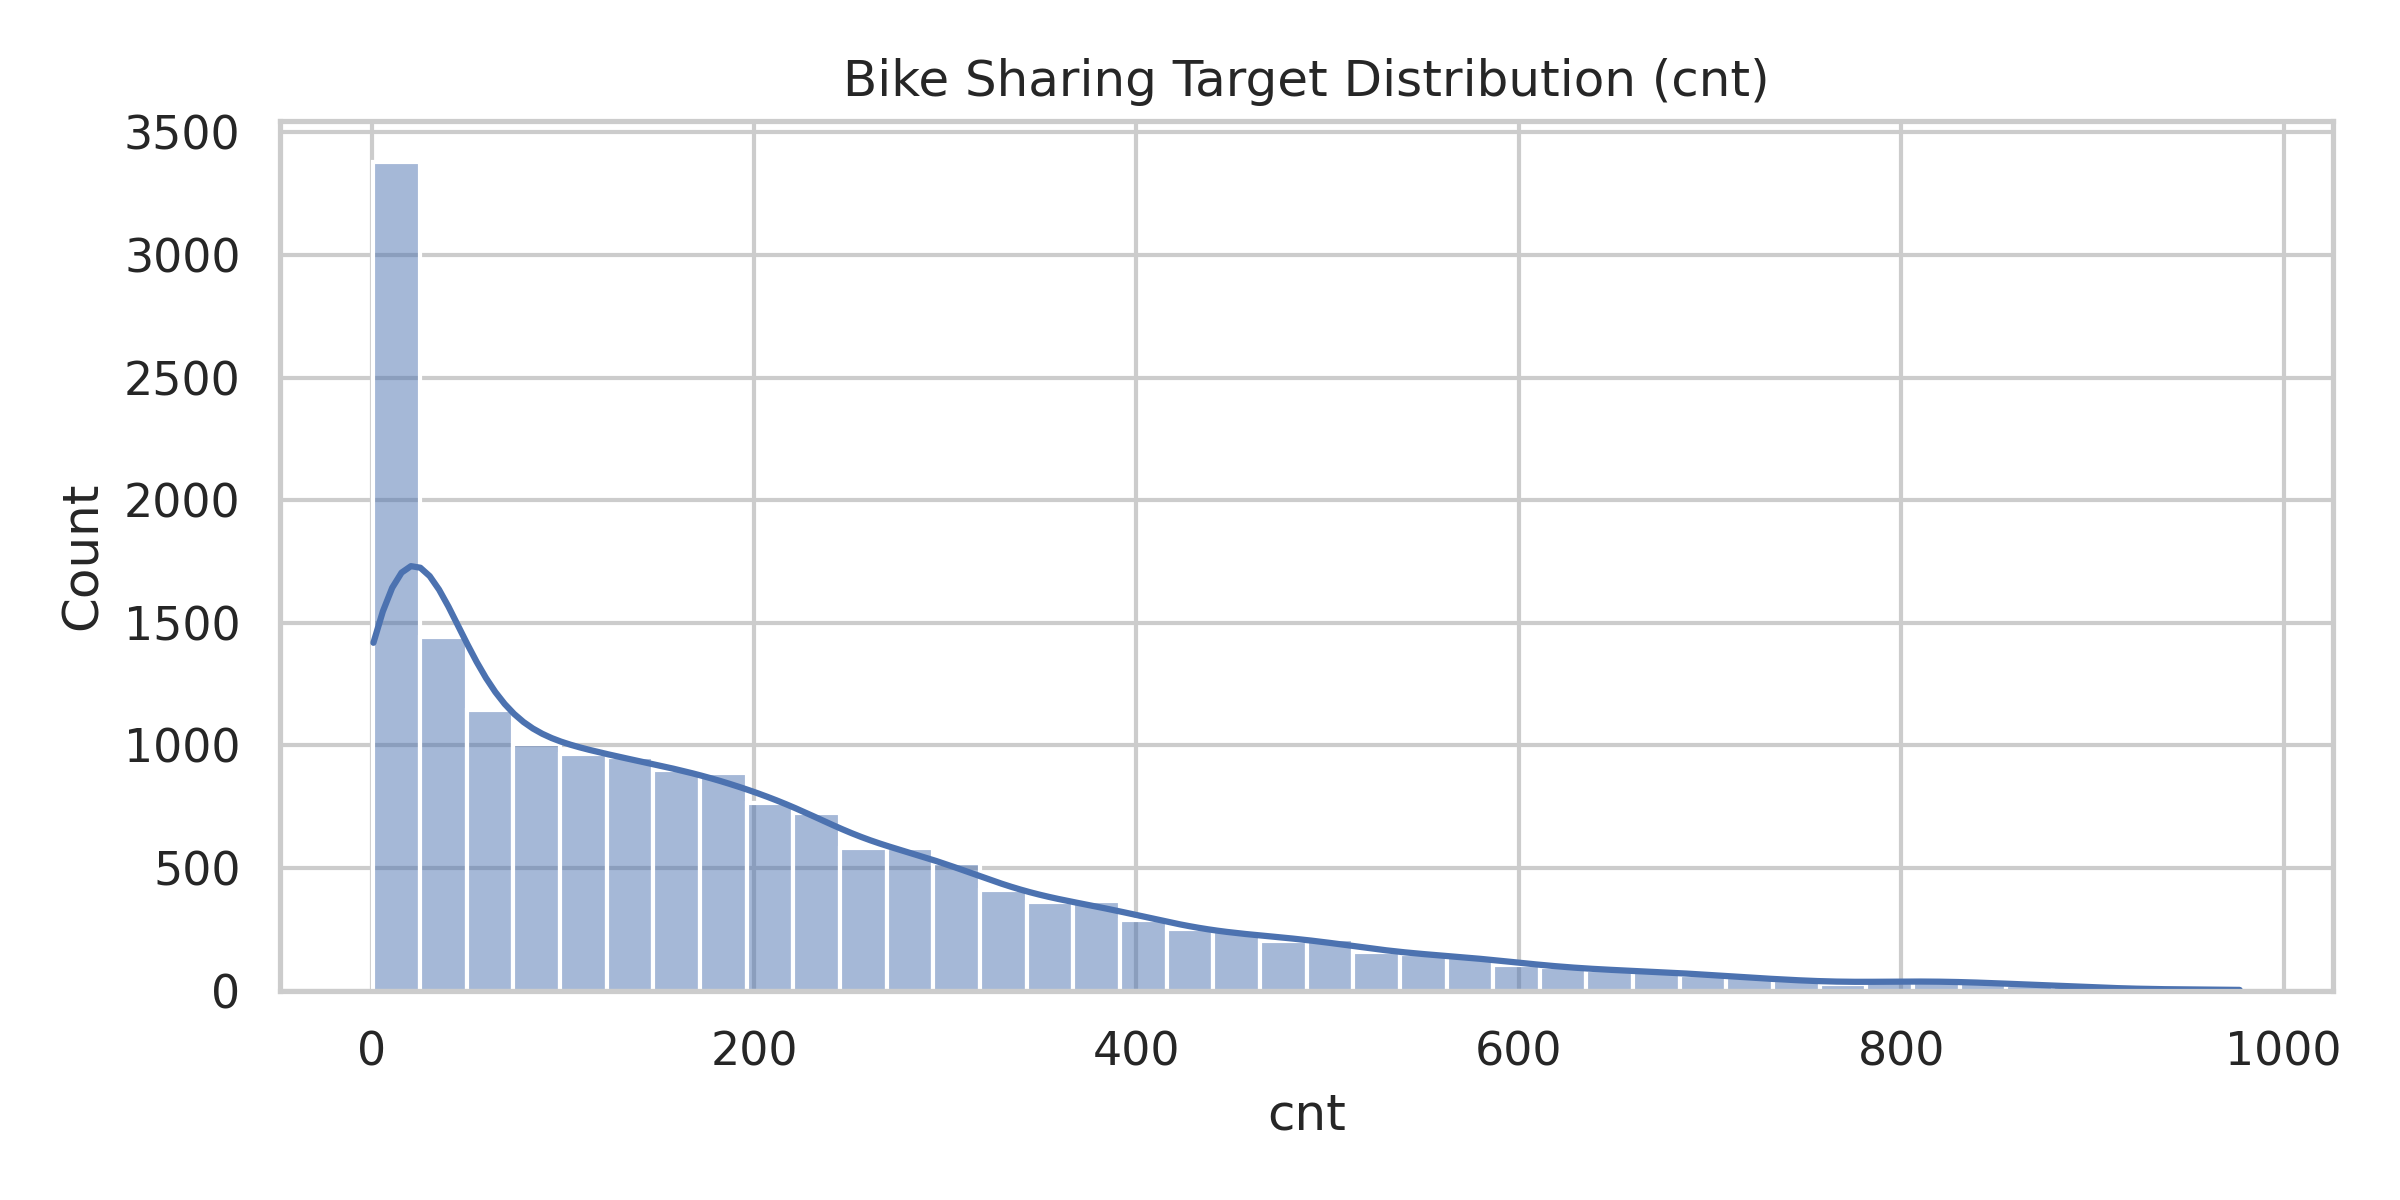
\includegraphics[width=0.65\textwidth]{../pre_study/figures/bike_sharing_target_distribution.png}\\[0.3em]
    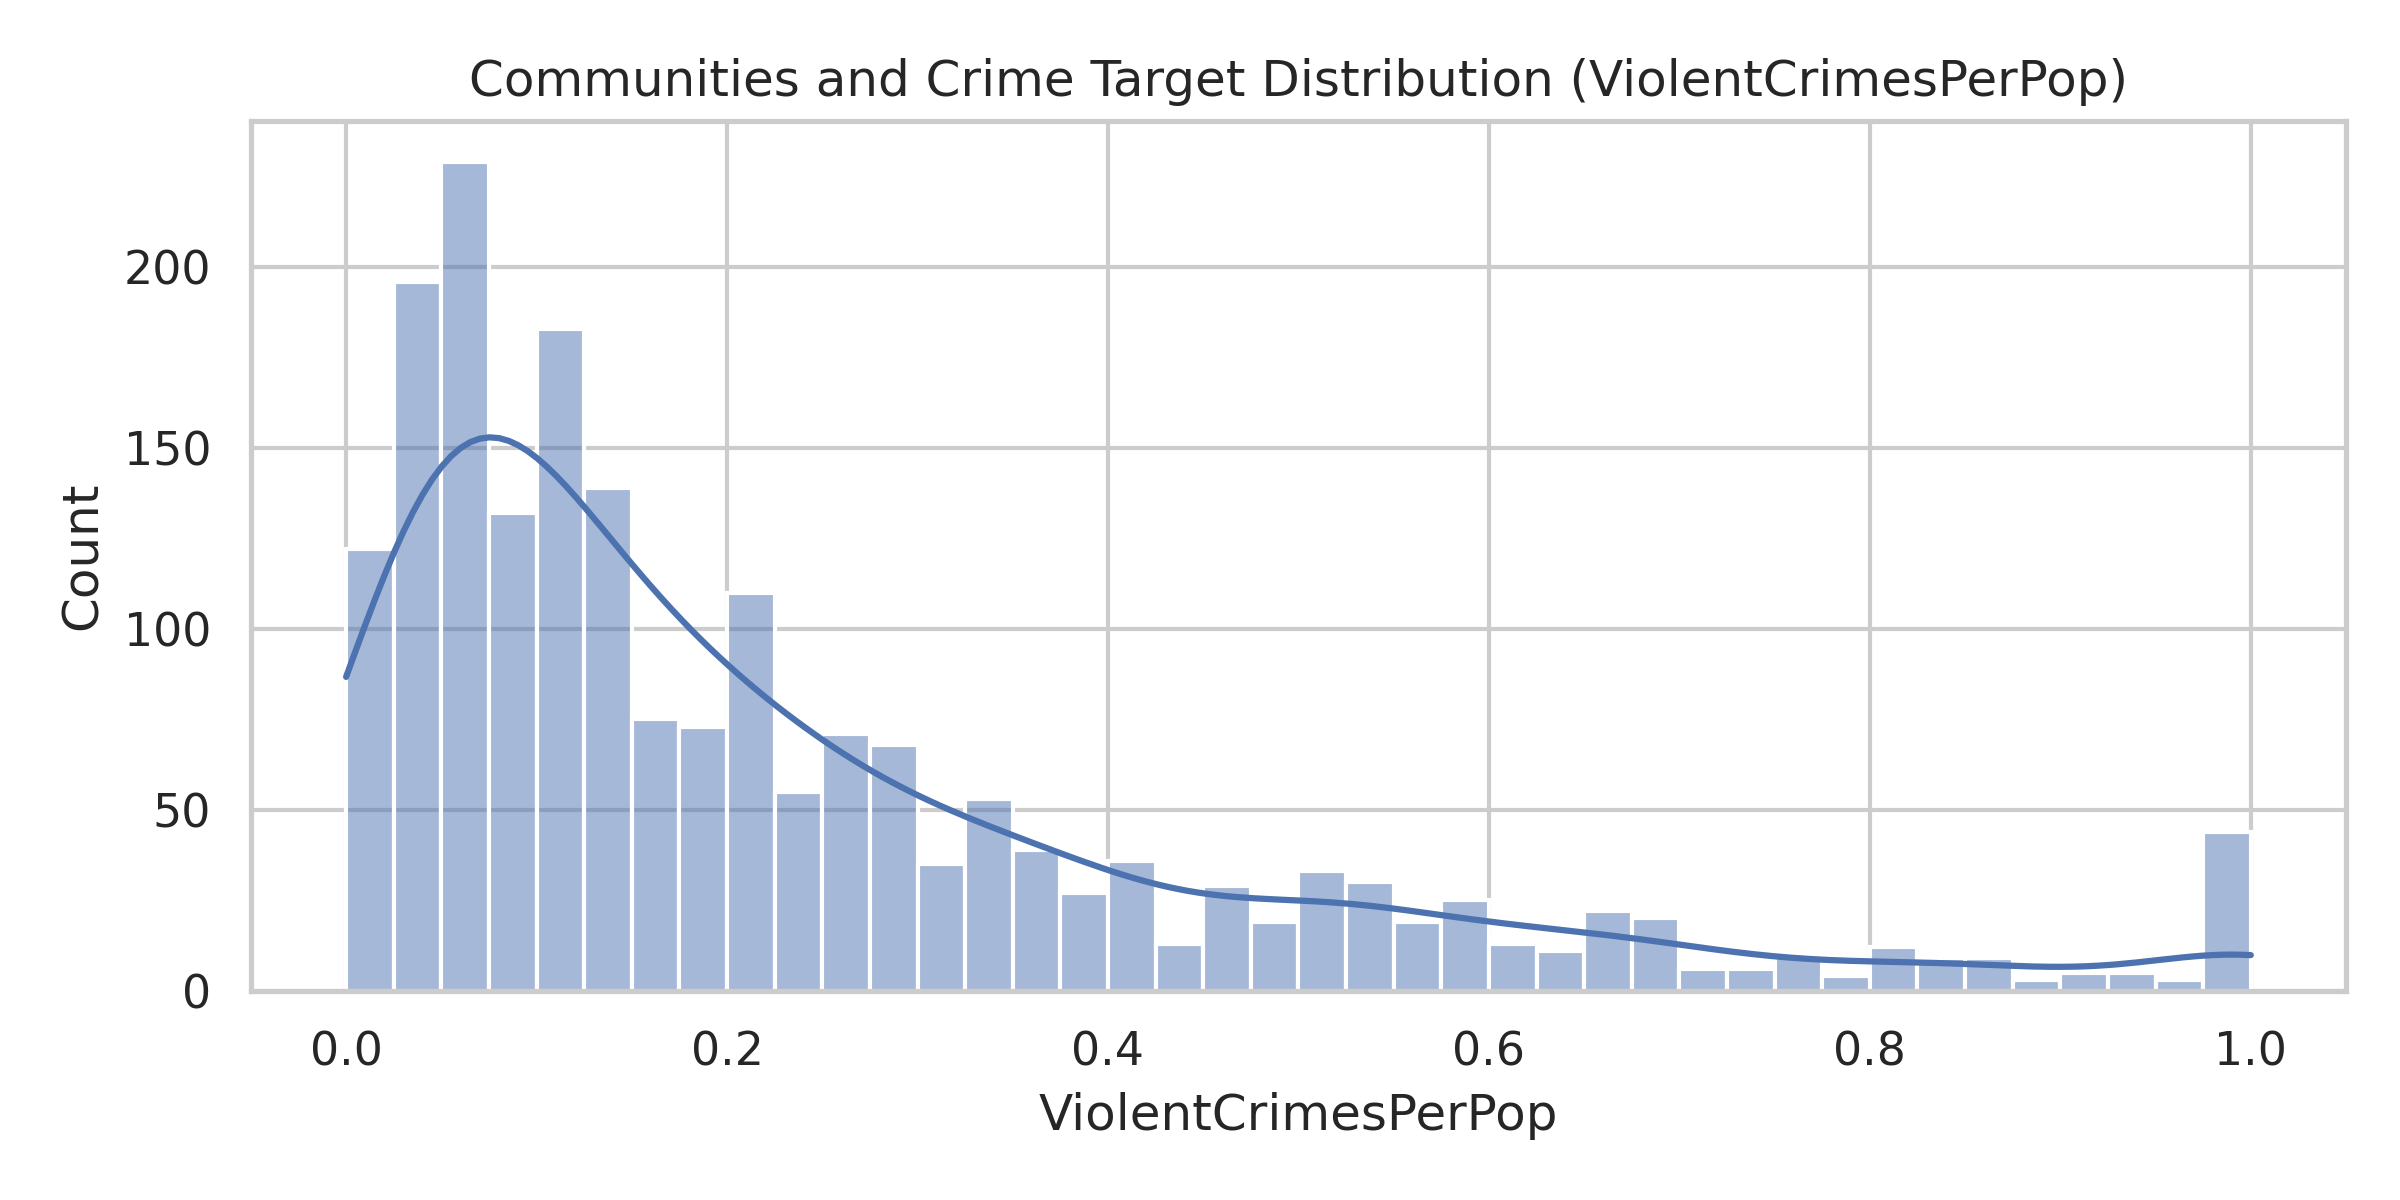
\includegraphics[width=0.65\textwidth]{../pre_study/figures/communities_crime_target_distribution.png}
    \caption{Target variable distributions for all four datasets.}
    \label{fig:target_dist}
\end{figure}

\begin{figure}[p]
    \centering
    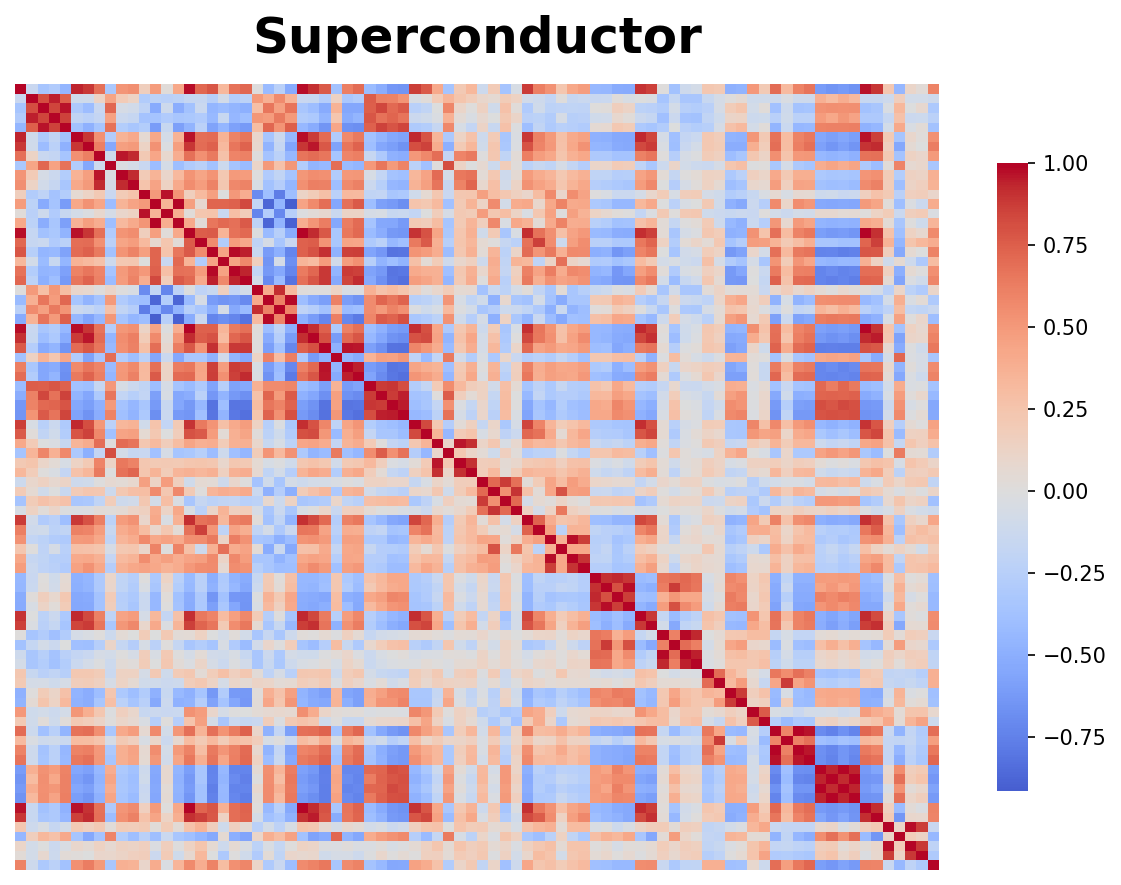
\includegraphics[width=0.48\textwidth]{../pre_study/figures/superconductor_correlation_heatmap.png}
    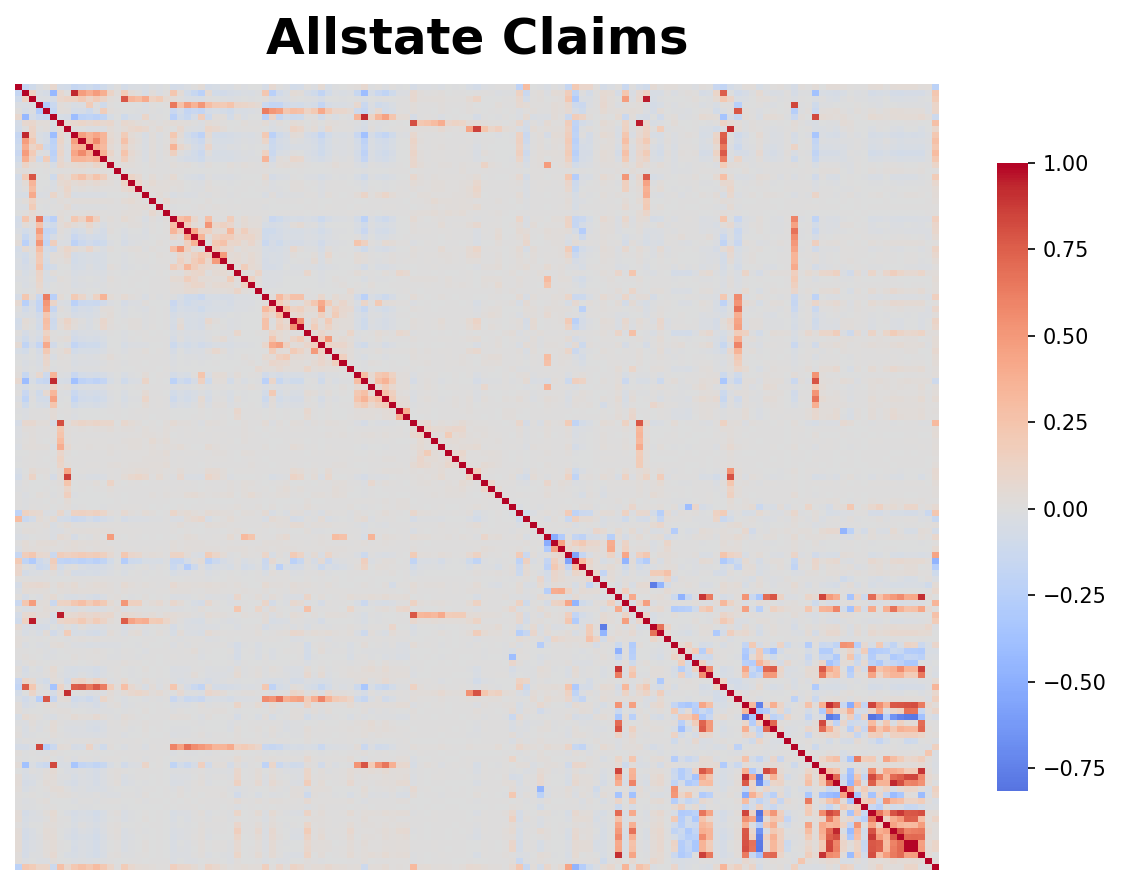
\includegraphics[width=0.48\textwidth]{../pre_study/figures/allstate_claims_correlation_heatmap.png}\\[0.5em]
    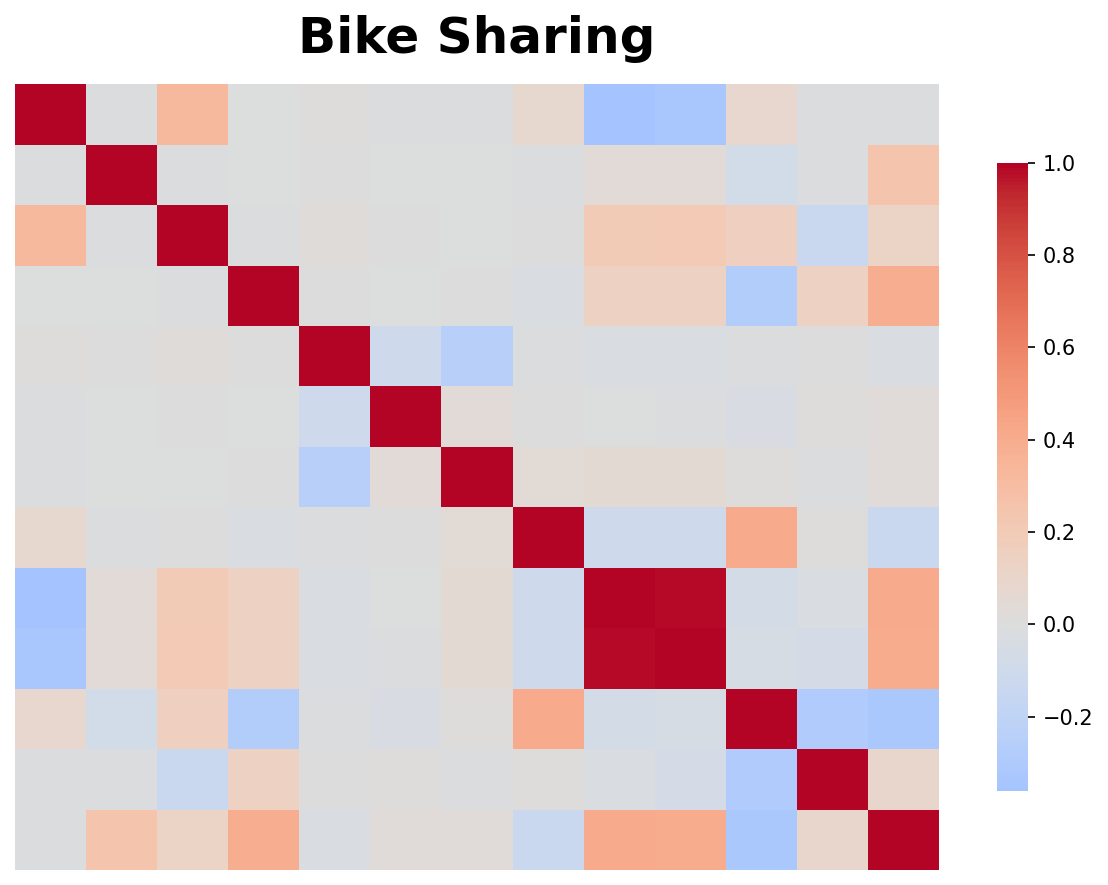
\includegraphics[width=0.48\textwidth]{../pre_study/figures/bike_sharing_correlation_heatmap.png}
    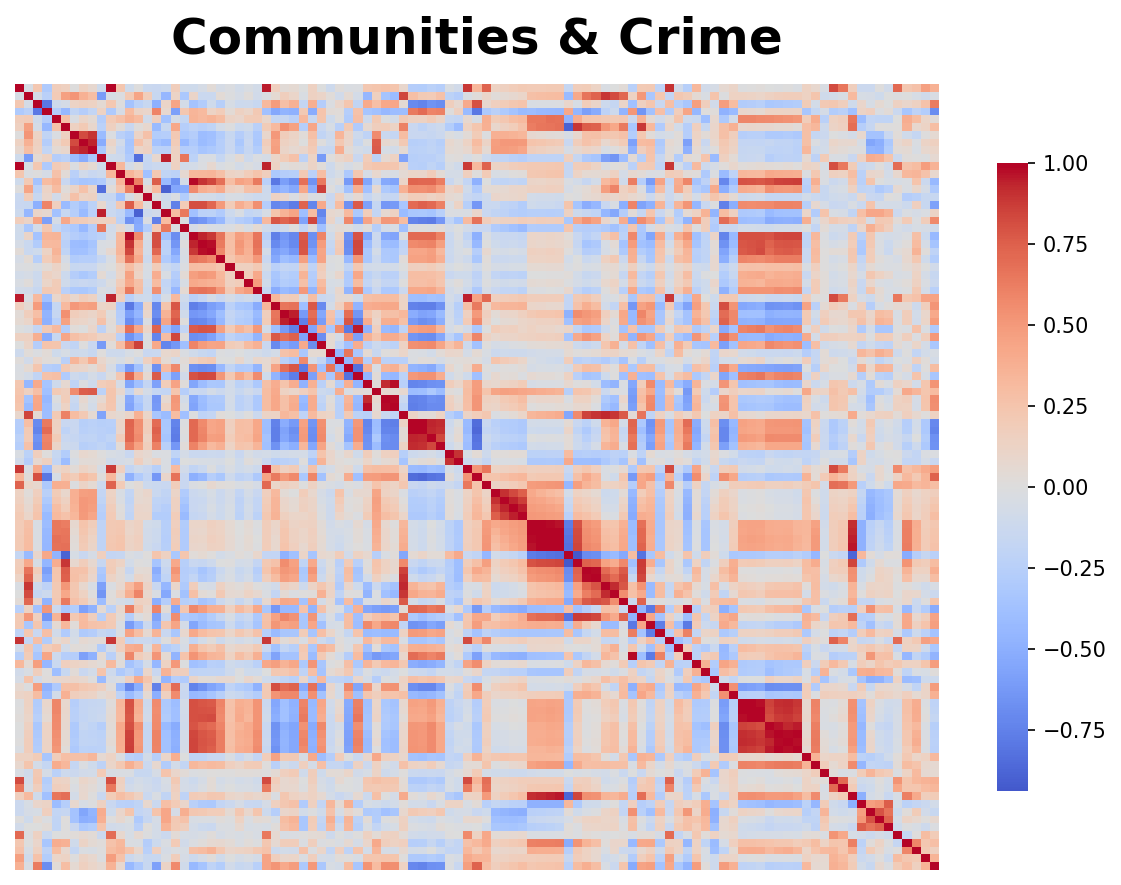
\includegraphics[width=0.48\textwidth]{../pre_study/figures/communities_crime_correlation_heatmap.png}
    \caption{Feature correlation heatmaps showing multicollinearity patterns across the four datasets.}
    \label{fig:correlation}
\end{figure}

\section{Chapter Summary}

This review has established the technical context for the experimental work. Regression on tabular data is best served by ensemble tree methods, though linear baselines remain useful references. Feature selection spans filter, wrapper, and embedded approaches, each with distinct trade-offs. SHAP provides theoretically principled feature attributions, and TreeExplainer makes exact computation tractable for tree models, though not without cost. The selected datasets span a meaningful range of sizes and structures, enabling evaluation of whether method performance generalizes. With this foundation in place, the next chapter formalizes the research hypotheses and experimental design.

\chapter{Research Hypotheses and Experimental Design}

This chapter formalizes the research questions motivating this thesis and describes the experimental protocol designed to address them. The approach follows a two-stage structure: a broad screening benchmark to map general behavior, followed by a focused deep dive to test SHAP-intensive strategies under controlled conditions.

\section{Research Questions}

The central inquiry of this thesis can be stated as:

\begin{quote}
\textit{Does SHAP-based feature selection provide practically relevant advantages over established alternatives when applied to tabular regression, considering predictive accuracy, selection stability, and computational cost jointly?}
\end{quote}

This question decomposes into several testable components:

\begin{enumerate}
    \item \textbf{Effectiveness}: Do SHAP-selected feature subsets yield lower prediction error than subsets chosen by standard methods?
    \item \textbf{Cost}: What computational overhead does SHAP-based selection incur, and does any performance gain justify this cost?
    \item \textbf{Stability}: Are SHAP-selected subsets consistent across repeated runs, or does the method introduce additional variability?
    \item \textbf{Generalization}: Do observed patterns hold across different datasets and model families, or are conclusions dataset-specific?
\end{enumerate}

\section{Hypotheses}

Based on the literature review and preliminary analysis, the following hypotheses guide the experimental work:

\subsection{H1: Competitive but Non-Dominant Performance}

In the broad benchmark across heterogeneous datasets and model families, SHAP-based feature selection will produce competitive prediction error compared to standard methods (mutual information, recursive feature elimination, tree-based importance), but will not be uniformly dominant. Different methods will excel on different dataset-model combinations, reflecting the no-free-lunch principle in feature selection.

\subsection{H2: Marginal Gains at Intermediate Retention}

In focused evaluation with XGBoost, SHAP-based recursive elimination and hybrid strategies may produce small improvements at intermediate feature retention levels (e.g., $k=0.25$ to $k=0.50$). At very low retention ($k < 0.15$), aggressive pruning may harm all methods; at full retention ($k=1.0$), selection becomes irrelevant.

\subsection{H3: Substantial Computational Overhead}

SHAP-intensive strategies, particularly those involving iterative SHAP computation (custom SHAP-RFE, hybrid pipelines), will require substantially higher selection time than native importance or simple filter methods.

\subsection{H4: Reduced Stability at Low Retention}

Selection stability will decrease as the retention ratio decreases, across all methods. However, SHAP-based methods may exhibit additional instability due to the stochastic nature of tree ensembles and the sensitivity of SHAP rankings to model refitting.

\section{Experimental Design}

The experimental protocol consists of two stages designed to balance breadth and depth.

\subsection{Stage 1: Broad Screening Benchmark}

The first stage surveys the landscape of feature selection performance across multiple datasets, models, and methods. This screening identifies general patterns and informs the selection of configurations for deeper analysis.

\textbf{Datasets}: The four datasets described in Chapter~2 (Allstate Claims, Bike Sharing, Communities and Crime, Superconductor) span a range of sizes and dimensionalities.

\textbf{Models}: Three model families are evaluated:
\begin{itemize}
    \item Ridge regression (linear baseline)
    \item ExtraTrees (bagging ensemble)
    \item XGBoost (gradient boosting)
\end{itemize}

\textbf{Feature selection strategies}:
\begin{itemize}
    \item Mutual Information (MI): filter method based on statistical dependency
    \item Recursive Feature Elimination (RFE): wrapper method with iterative removal
    \item Tree-based Importance (Tree-FI): embedded method using native importance
    \item SHAP-based Importance: ranking by mean absolute SHAP value
\end{itemize}

\textbf{Feature retention levels}: Selection is evaluated at $k \in \{0.25, 0.50, 0.75, 1.00\}$, where $k$ represents the proportion of original features retained.

\textbf{Evaluation}: Each configuration is run with cross-validation to obtain robust error estimates. Metrics include RMSE (primary), MAE, and MAPE. Selection time and total execution time are recorded.

\subsection{Stage 2: Focused Deep Dive}

The second stage narrows focus to XGBoost---the model family showing consistently strong and operationally relevant performance in Stage~1---and tests more sophisticated SHAP-based strategies.

\textbf{Datasets}: Two datasets are selected for focused analysis:
\begin{itemize}
    \item Superconductor: moderate scale, dense numeric structure
    \item Allstate Claims: large scale, high dimensional
\end{itemize}

\textbf{Selection strategies}:
\begin{itemize}
    \item \texttt{native\_fi}: XGBoost native feature importance ranking
    \item \texttt{custom\_shap\_rfe}: recursive elimination guided by SHAP scores, removing features iteratively until the target retention is reached
    \item \texttt{hybrid\_fi\_custom\_shap\_rfe}: initial pruning using native importance to reduce the feature set, followed by SHAP-guided recursive elimination on the reduced set
    \item \texttt{baseline}: no selection, all features retained ($k=1.0$)
\end{itemize}

\textbf{Feature retention levels}: A finer grid is used: $k \in \{0.05, 0.10, 0.15, 0.25, 0.50, 1.00\}$.

\textbf{Additional metrics}: Beyond prediction error and timing, Stage~2 tracks selection stability via Jaccard similarity between feature subsets across runs, and multicollinearity indicators in the selected subsets.

\subsection{Rationale for Two-Stage Design}

A direct exhaustive comparison of all methods across all datasets with fine-grained retention levels would be computationally prohibitive and produce unwieldy results. The two-stage approach serves multiple purposes:

\begin{enumerate}
    \item \textbf{Feasibility}: Stage~1 provides broad coverage with coarse granularity; Stage~2 invests computation where it matters most.
    \item \textbf{Focus}: By narrowing to XGBoost in Stage~2, method effects are isolated from model-family effects.
    \item \textbf{Relevance}: The hybrid and custom SHAP-RFE strategies are more computationally intensive; testing them on selected configurations ensures practical relevance of the comparison.
\end{enumerate}

\section{Evaluation Metrics}

Assessment is structured around three axes, reflecting the thesis objective of evaluating practical utility:

\textbf{Predictive effectiveness}: Root Mean Squared Error (RMSE) serves as the primary metric, supplemented by Mean Absolute Error (MAE) and Mean Absolute Percentage Error (MAPE). Lower values indicate better performance.

\textbf{Selection stability}: Measured by Jaccard similarity between feature subsets selected in different cross-validation folds or repeated runs. Values range from 0 (no overlap) to 1 (identical subsets). Higher stability suggests more robust selection.

\textbf{Computational cost}: Measured by selection time (time spent on feature selection) and total execution time (selection plus model training and evaluation). Costs are compared in absolute terms and as ratios between methods.

Comparisons are always interpreted as trade-offs. A method that achieves marginally lower RMSE but requires dramatically higher computation may not be practically preferable.

\section{Implementation and Reproducibility}

All experiments are implemented in Python using scikit-learn, XGBoost, and the SHAP library. The experimental pipeline is modular, with separate components for data loading, feature selection, model training, evaluation, and result persistence.

Cross-validation uses a fixed number of folds with reproducible random seeds. Results are saved as raw CSV files containing per-fold metrics, along with aggregated summaries. Figures are generated programmatically to ensure consistency.

\section{Chapter Summary}

This chapter has established the hypotheses driving the experimental work and described a two-stage protocol designed to evaluate SHAP-based feature selection systematically. The broad screening stage covers multiple datasets and models to identify general patterns, while the focused deep dive tests SHAP-intensive strategies where they are most likely to show value. Evaluation emphasizes practical trade-offs among effectiveness, stability, and cost. The next chapter presents the experimental execution and results.

\chapter{Experimental Results and Analysis}

This chapter reports the outcomes of the two experimental stages and analyzes the findings against the hypotheses established in Chapter~3. The presentation follows the experimental structure: first the broad screening results from Stage~1, then the focused deep-dive results from Stage~2, and finally a synthesis of findings across both stages.

\section{Stage 1: Broad Screening Results}

Stage~1 evaluated four feature selection strategies across four datasets and three model families, producing 7,920 individual observations in the summarized outputs. This section presents aggregate findings organized by research question.

\subsection{Predictive Performance}

Table~\ref{tab:stage1_best} reports the best-performing strategy for each dataset-model combination, determined by minimum mean RMSE across all retention levels.

\begin{table}[h]
\centering
\caption{Best RMSE by dataset and model in Stage~1, showing winning strategy and retention level.}
\label{tab:stage1_best}
\begin{tabular}{llllr}
\toprule
\textbf{Dataset} & \textbf{Model} & \textbf{Best Strategy} & \textbf{k} & \textbf{RMSE} \\
\midrule
Allstate Claims & Ridge & MI & 1.00 & 2090.07 \\
Allstate Claims & ExtraTrees & MI & 1.00 & 1992.76 \\
Allstate Claims & XGBoost & SHAP & 0.50 & 1897.11 \\
\midrule
Bike Sharing & Ridge & MI & 1.00 & 141.04 \\
Bike Sharing & ExtraTrees & MI & 1.00 & 40.83 \\
Bike Sharing & XGBoost & MI & 1.00 & 42.57 \\
\midrule
Communities \& Crime & Ridge & MI & 1.00 & 0.136 \\
Communities \& Crime & ExtraTrees & Tree-FI & 0.50 & 0.134 \\
Communities \& Crime & XGBoost & SHAP & 0.75 & 0.138 \\
\midrule
Superconductor & Ridge & MI & 1.00 & 17.65 \\
Superconductor & ExtraTrees & MI & 0.75 & 9.11 \\
Superconductor & XGBoost & Tree-FI & 0.75 & 9.98 \\
\bottomrule
\end{tabular}
\end{table}

Several patterns emerge from this summary:

\textbf{No universal winner}: As hypothesized (H1), no single strategy dominates all configurations. The winning method varies by dataset and model, confirming that feature selection effectiveness is context-dependent.

\textbf{MI frequently competitive}: Mutual Information achieves the best result in 7 of 12 configurations, often at $k=1.00$ (full feature set). This suggests that for some dataset-model pairs, feature selection provides no benefit over using all features, and MI's ranking at least does not harm performance.

\textbf{SHAP wins selectively}: SHAP achieves the best RMSE in 2 configurations, both with XGBoost---Allstate at $k=0.50$ and Communities and Crime at $k=0.75$. These wins occur at intermediate retention levels, consistent with hypothesis H2.

\textbf{Tree-FI competitive for tree models}: Tree-based importance wins in 2 configurations, both with tree-based models (ExtraTrees on Communities, XGBoost on Superconductor).

Figure~\ref{fig:stage1_rmse} visualizes RMSE by strategy across datasets, illustrating the variability in method rankings.

\begin{figure}[h]
    \centering
    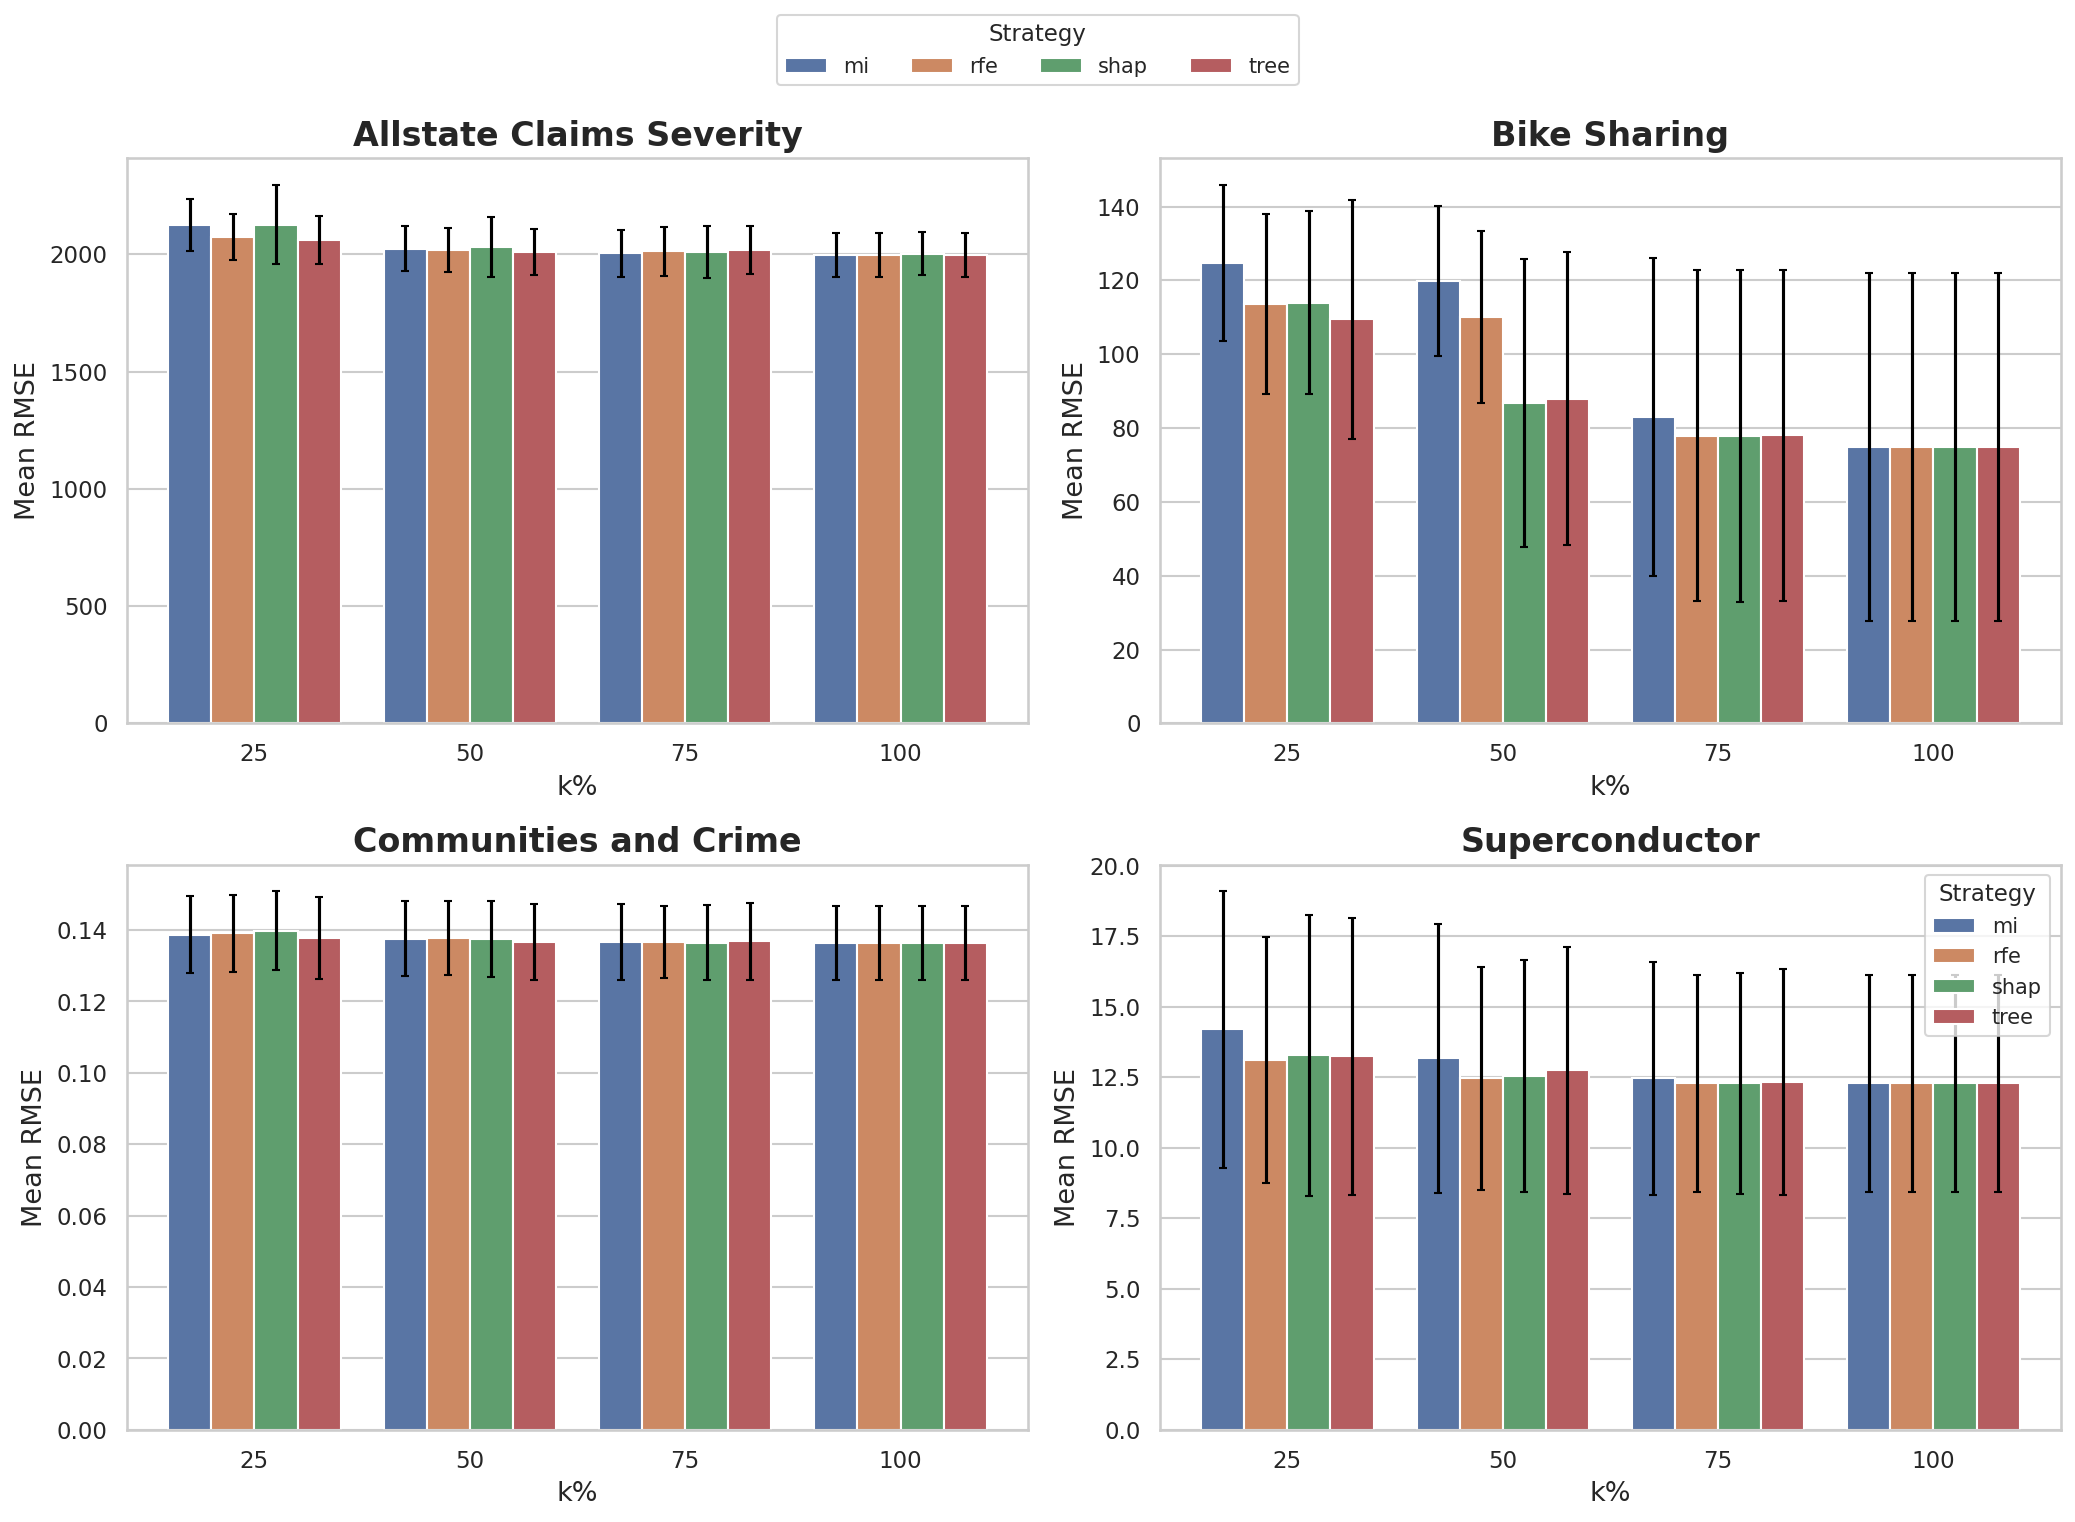
\includegraphics[width=0.85\textwidth]{../runs/exp1_plus_big-arff-run/figures/fig1_rmse_by_strategy_all_2x2.png}
    \caption{Stage~1 RMSE comparison by strategy across all four datasets.}
    \label{fig:stage1_rmse}
\end{figure}

\subsection{Computational Cost}

Table~\ref{tab:stage1_cost} presents average selection time by strategy and model family, aggregated across datasets and retention levels.

\begin{table}[h]
\centering
\caption{Mean selection time (seconds) by strategy and model in Stage~1.}
\label{tab:stage1_cost}
\begin{tabular}{lrrr}
\toprule
\textbf{Strategy} & \textbf{Ridge} & \textbf{ExtraTrees} & \textbf{XGBoost} \\
\midrule
MI & 0.75 & 0.82 & 0.72 \\
RFE & 0.27 & 0.16 & 0.26 \\
Tree-FI & 0.60 & 0.77 & 0.53 \\
SHAP & 0.01 & 5.42 & 0.54 \\
\bottomrule
\end{tabular}
\end{table}

The cost patterns reveal nuance: SHAP selection time varies dramatically by model. For Ridge, SHAP computation is near-instantaneous (linear SHAP is fast). For ExtraTrees, SHAP incurs substantial overhead---roughly 6-7x the cost of MI. For XGBoost, the TreeExplainer efficiency keeps SHAP competitive with other methods.

Figure~\ref{fig:stage1_cost} shows the full distribution of computational costs across configurations.

\begin{figure}[h]
    \centering
    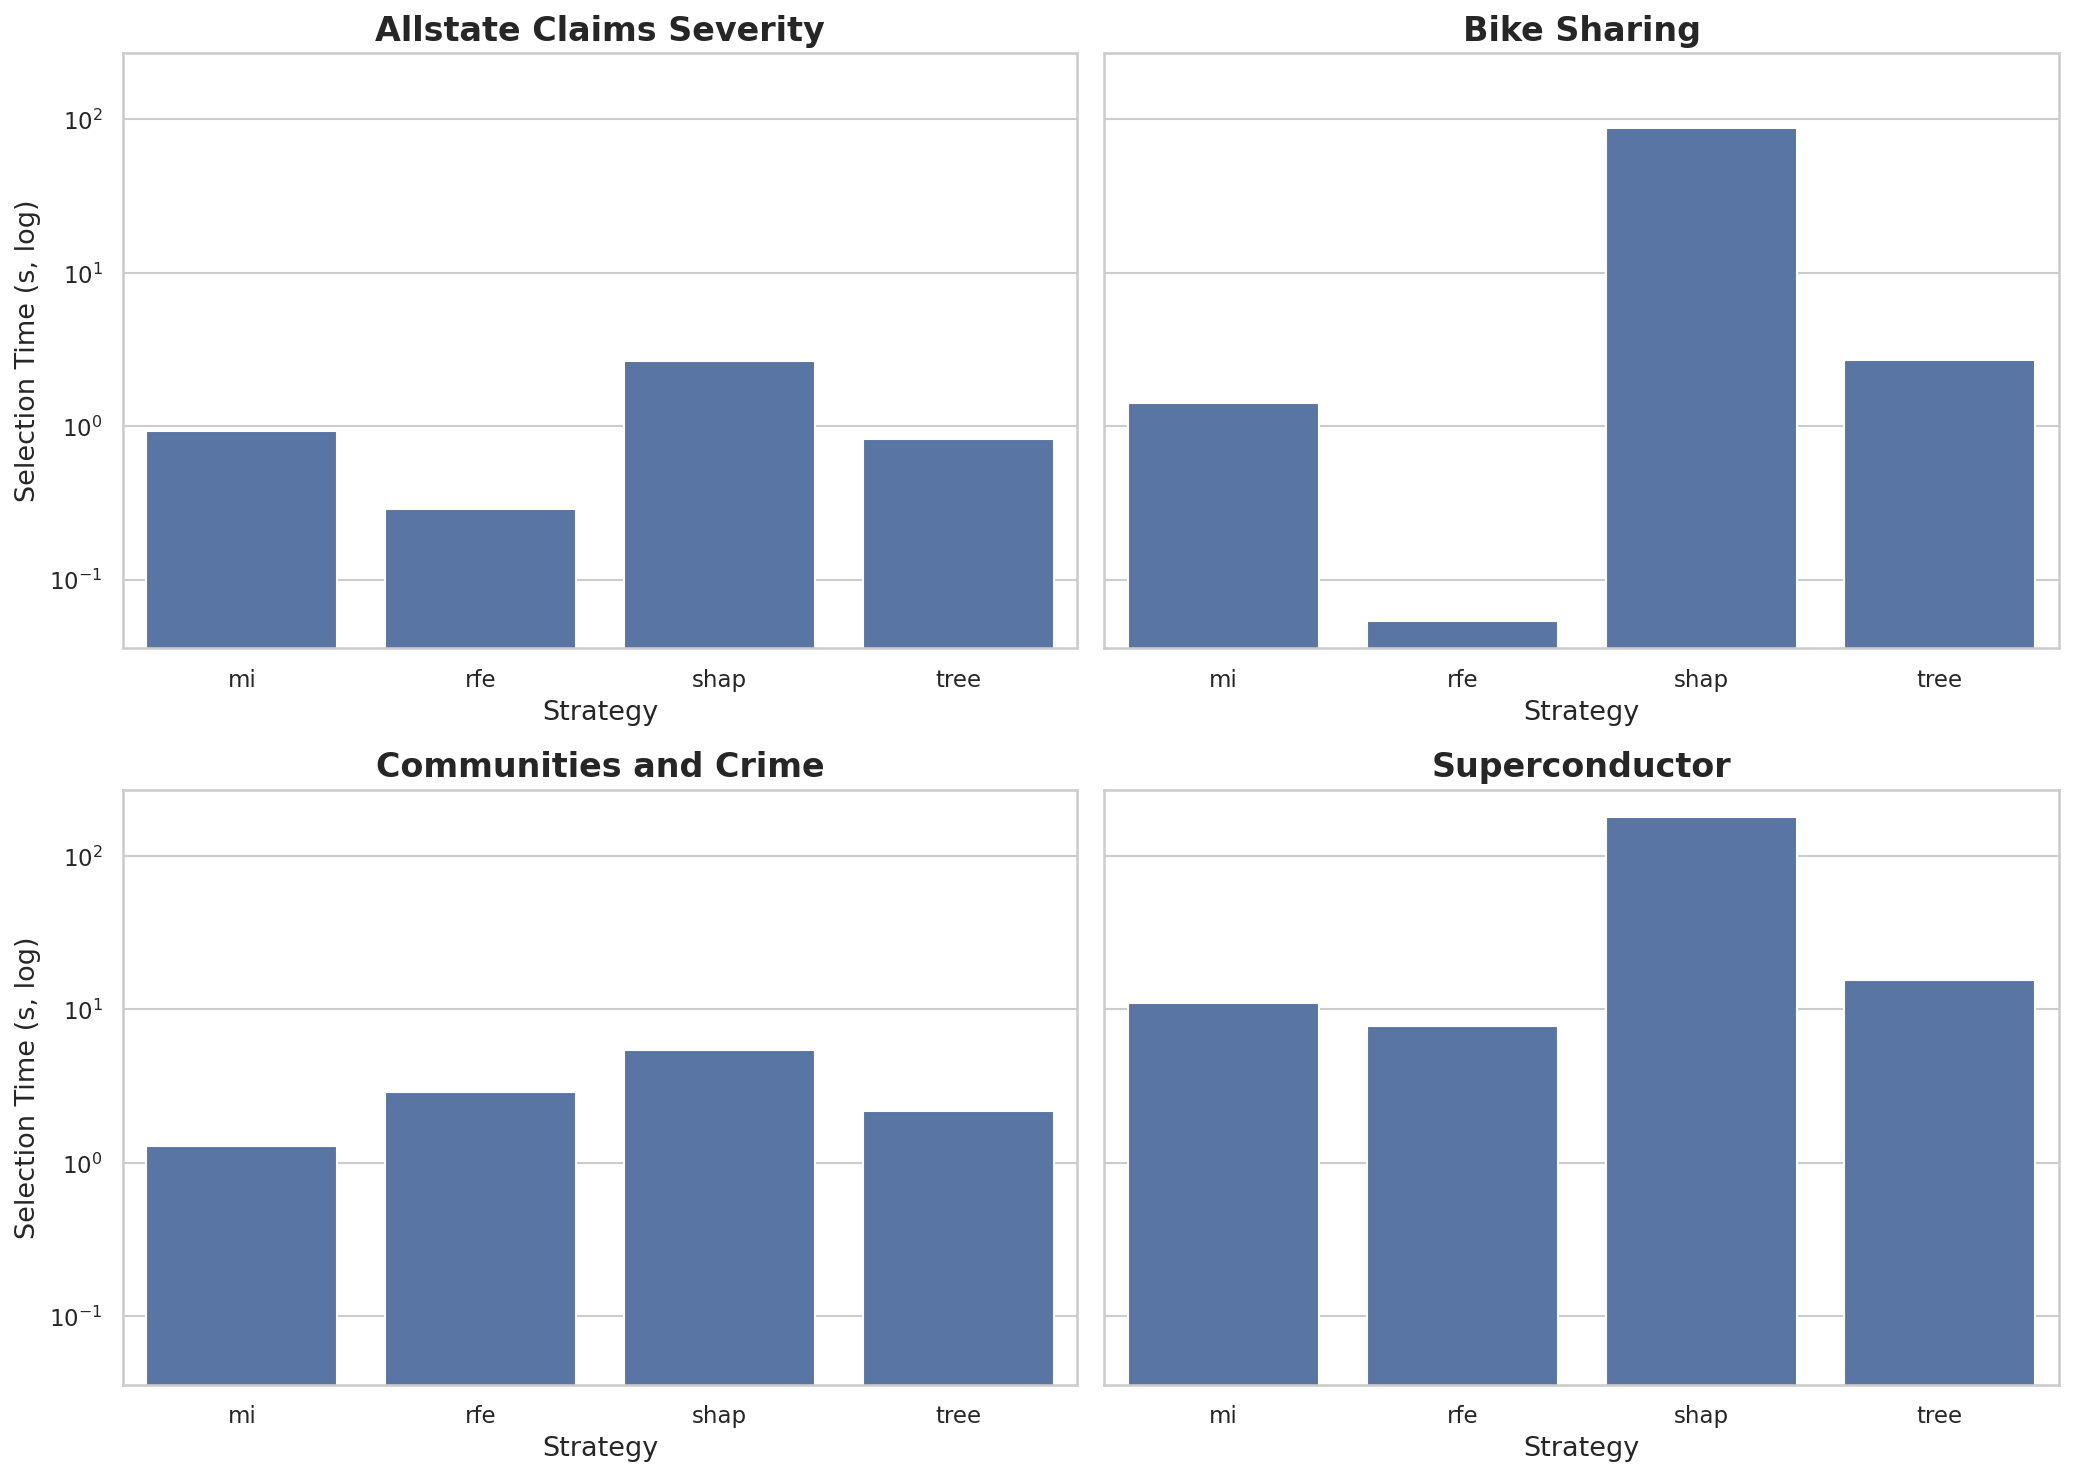
\includegraphics[width=0.85\textwidth]{../runs/exp1_plus_big-arff-run/figures/fig3_compute_cost_all_2x2.png}
    \caption{Stage~1 computational cost by strategy and dataset.}
    \label{fig:stage1_cost}
\end{figure}

\subsection{Selection Stability}

Table~\ref{tab:stage1_stability} summarizes Jaccard stability scores by strategy and retention level, averaged across datasets.

\begin{table}[h]
\centering
\caption{Mean Jaccard stability by strategy and retention level in Stage~1.}
\label{tab:stage1_stability}
\begin{tabular}{lrrrr}
\toprule
\textbf{Strategy} & \textbf{k=0.25} & \textbf{k=0.50} & \textbf{k=0.75} & \textbf{k=1.00} \\
\midrule
MI & 0.81 & 0.83 & 0.96 & 1.00 \\
RFE & 0.73 & 0.79 & 1.00 & 1.00 \\
SHAP & 0.63 & 0.77 & 0.97 & 1.00 \\
Tree-FI & 0.75 & 0.87 & 0.95 & 1.00 \\
\bottomrule
\end{tabular}
\end{table}

Stability increases with retention level across all methods, as expected---larger subsets have more overlap by construction. At $k=0.25$, SHAP shows the lowest stability (0.63), supporting hypothesis H4 that SHAP-based selection may introduce additional variability. By $k=0.75$, all methods converge to high stability.

\subsection{Stage 1 Summary}

The broad screening confirms that SHAP-based selection can be competitive but is not systematically superior. XGBoost emerges as the most consistent performer among models, making it the natural choice for the focused Stage~2 analysis. The computational overhead of SHAP depends heavily on the model family, with TreeExplainer providing efficiency for gradient boosting.

\section{Stage 2: Focused Deep-Dive Results}

Stage~2 applies three feature selection strategies plus a baseline to XGBoost on two selected datasets: Superconductor and Allstate Claims. A finer retention grid ($k \in \{0.05, 0.10, 0.15, 0.25, 0.50, 1.00\}$) enables more detailed analysis.

\subsection{Superconductor Dataset}

Table~\ref{tab:stage2_super} presents RMSE and total time for each strategy and retention level on the Superconductor dataset.

\begin{table}[h]
\centering
\caption{Superconductor results: RMSE and total time by strategy and retention level.}
\label{tab:stage2_super}
\begin{tabular}{llrr}
\toprule
\textbf{Strategy} & \textbf{k} & \textbf{RMSE} & \textbf{Time (s)} \\
\midrule
native\_fi & 0.05 & 13.44 & 4.02 \\
custom\_shap\_rfe & 0.05 & 13.48 & 3.99 \\
hybrid & 0.05 & 13.51 & 98.18 \\
\midrule
native\_fi & 0.10 & 11.20 & 4.07 \\
custom\_shap\_rfe & 0.10 & 11.10 & 4.02 \\
hybrid & 0.10 & 11.15 & 100.79 \\
\midrule
native\_fi & 0.25 & 10.30 & 4.19 \\
custom\_shap\_rfe & 0.25 & 10.35 & 4.14 \\
hybrid & 0.25 & 10.34 & 111.08 \\
\midrule
native\_fi & 0.50 & 10.08 & 4.29 \\
custom\_shap\_rfe & 0.50 & 10.06 & 4.28 \\
hybrid & 0.50 & 10.05 & 130.76 \\
\midrule
baseline & 1.00 & 9.94 & 4.51 \\
\bottomrule
\end{tabular}
\end{table}

Key observations:

\textbf{Baseline wins at full retention}: The best absolute RMSE (9.94) is achieved with all features retained, suggesting that for this dataset, feature selection does not improve over the full model.

\textbf{Marginal differences between selection strategies}: At each retention level, native\_fi, custom\_shap\_rfe, and hybrid produce nearly identical RMSE (differences $<0.1$). The sophisticated SHAP-based approaches do not outperform simple native importance.

\textbf{Dramatic cost difference}: The hybrid strategy requires 25-30x more time than native\_fi or custom\_shap\_rfe at comparable retention levels. For a $<0.1$ RMSE difference that sometimes favors simpler methods, this overhead is difficult to justify.

Figure~\ref{fig:stage2_super} visualizes the RMSE-time trade-off.

\begin{figure}[h]
    \centering
    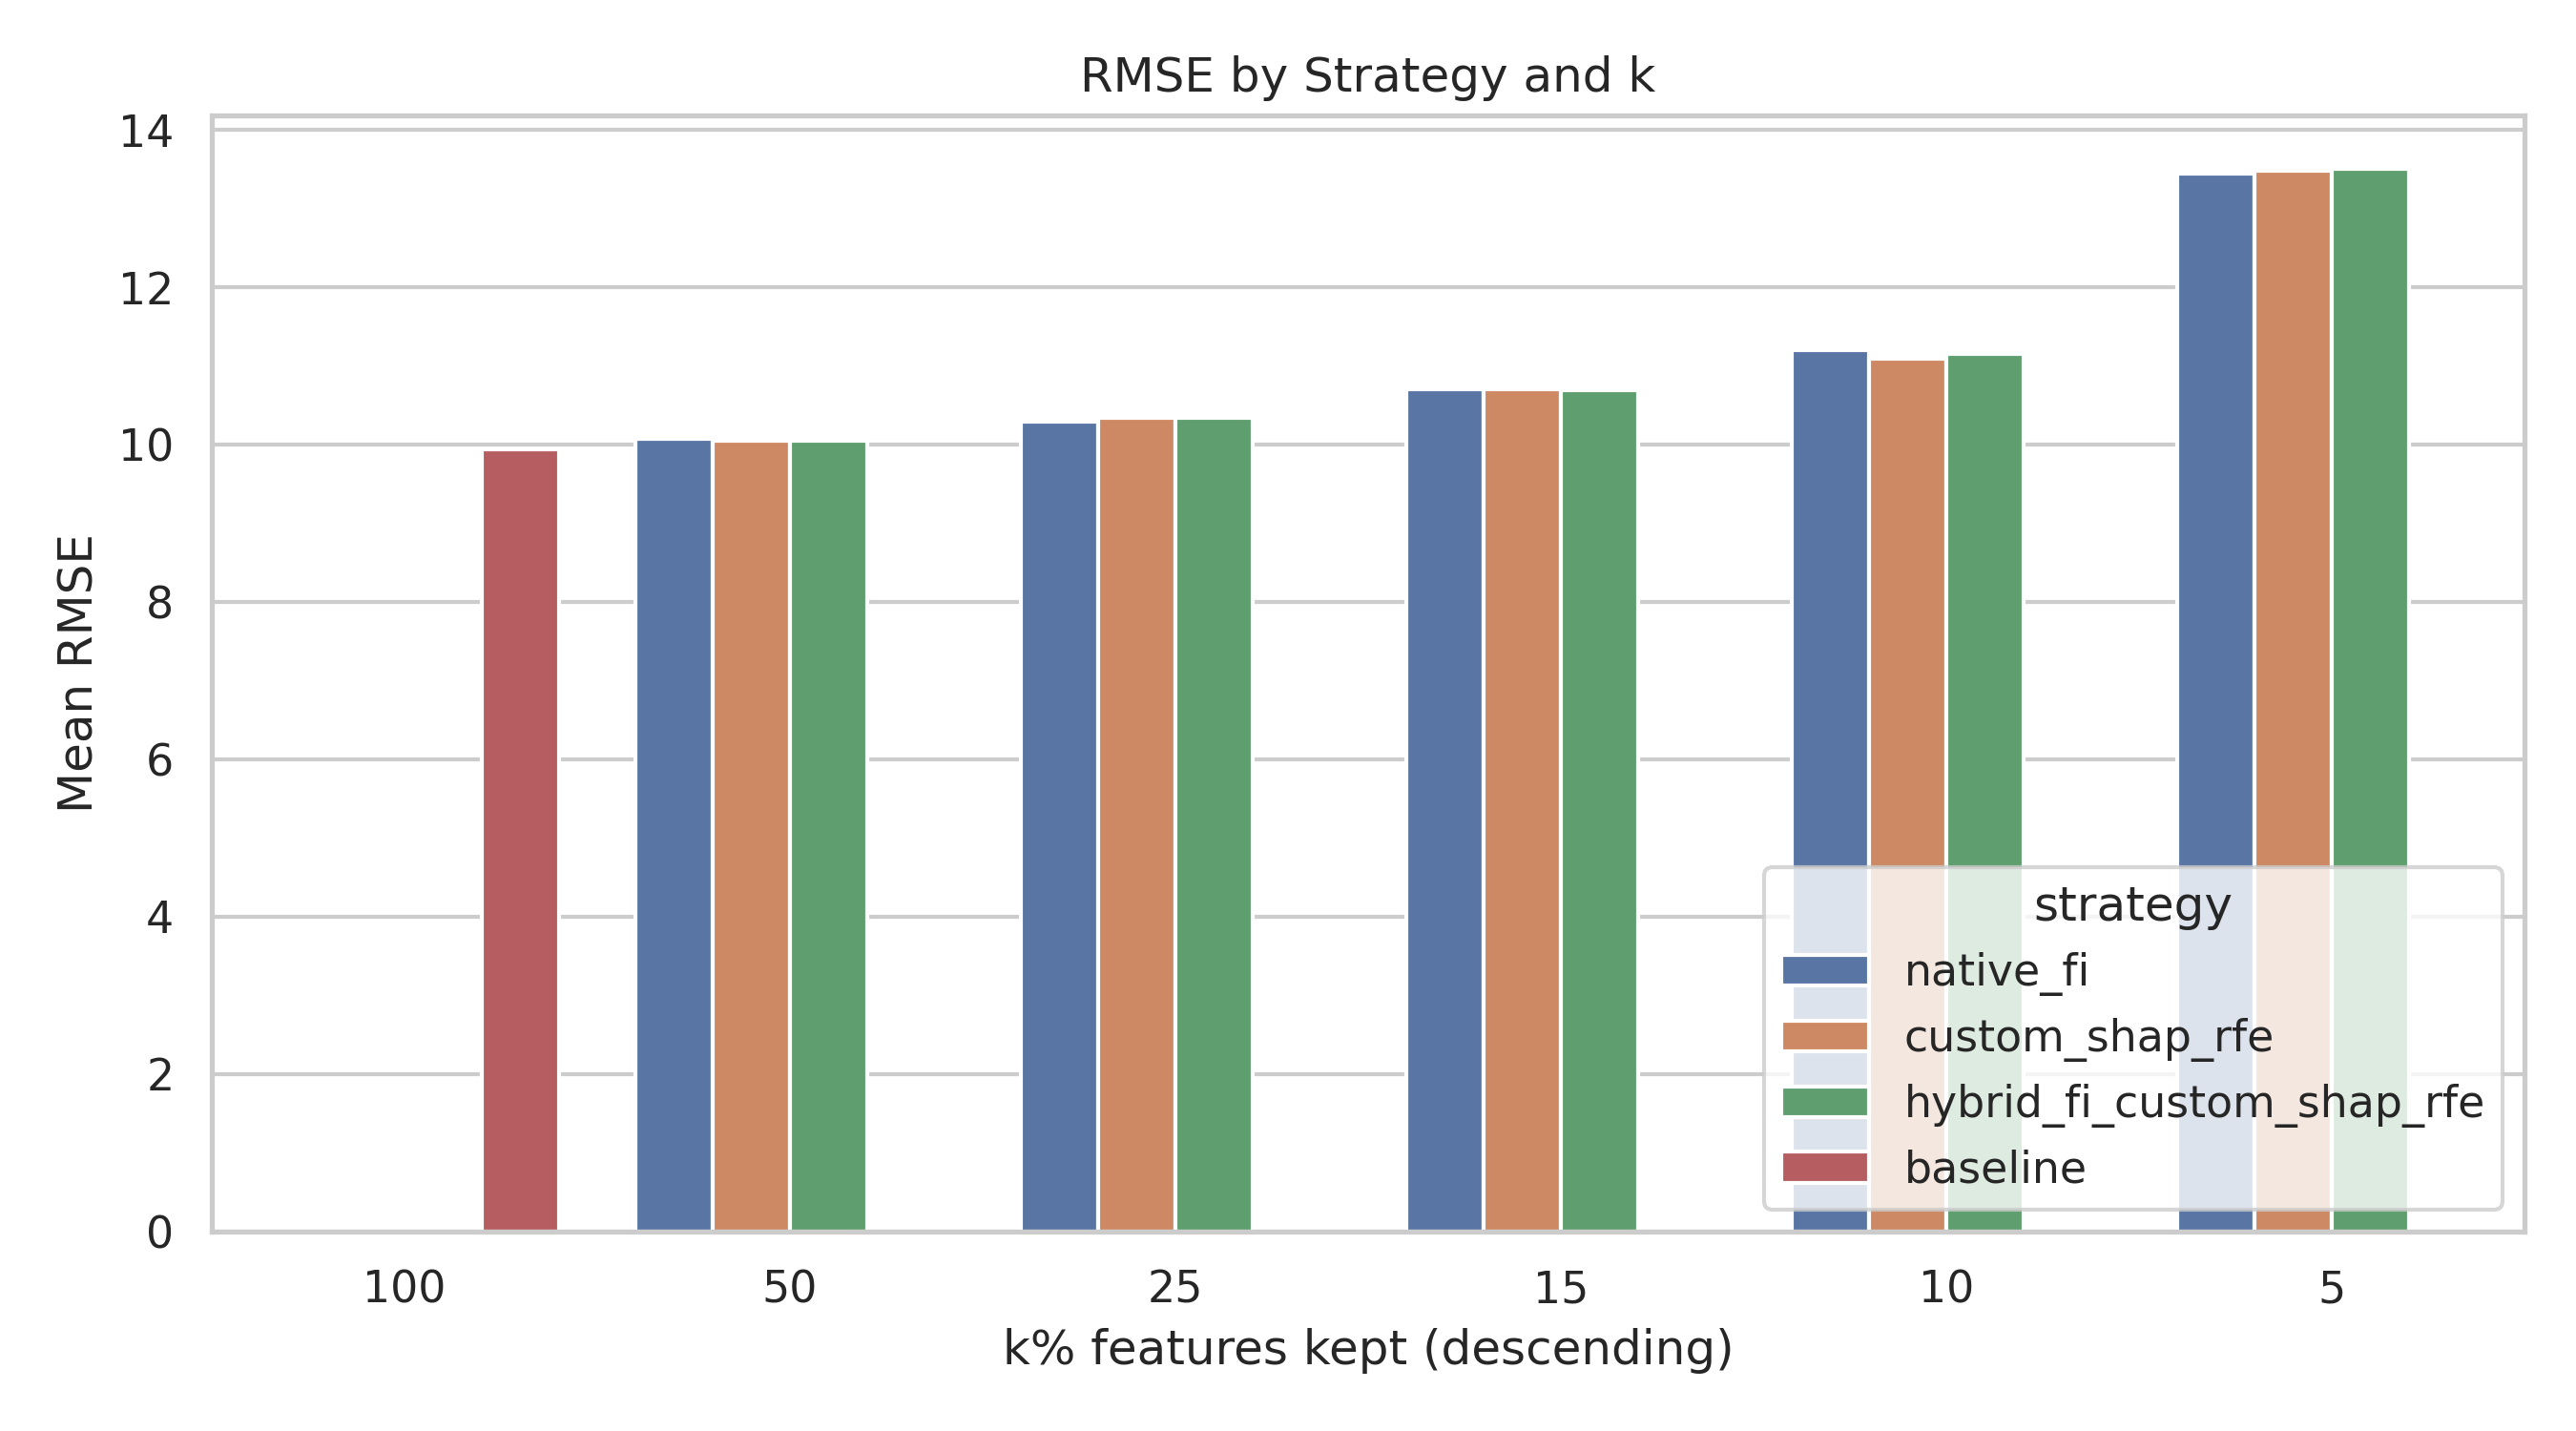
\includegraphics[width=0.48\textwidth]{../runs/exp2_run12/figures/exp2_rmse_by_strategy_k.png}
    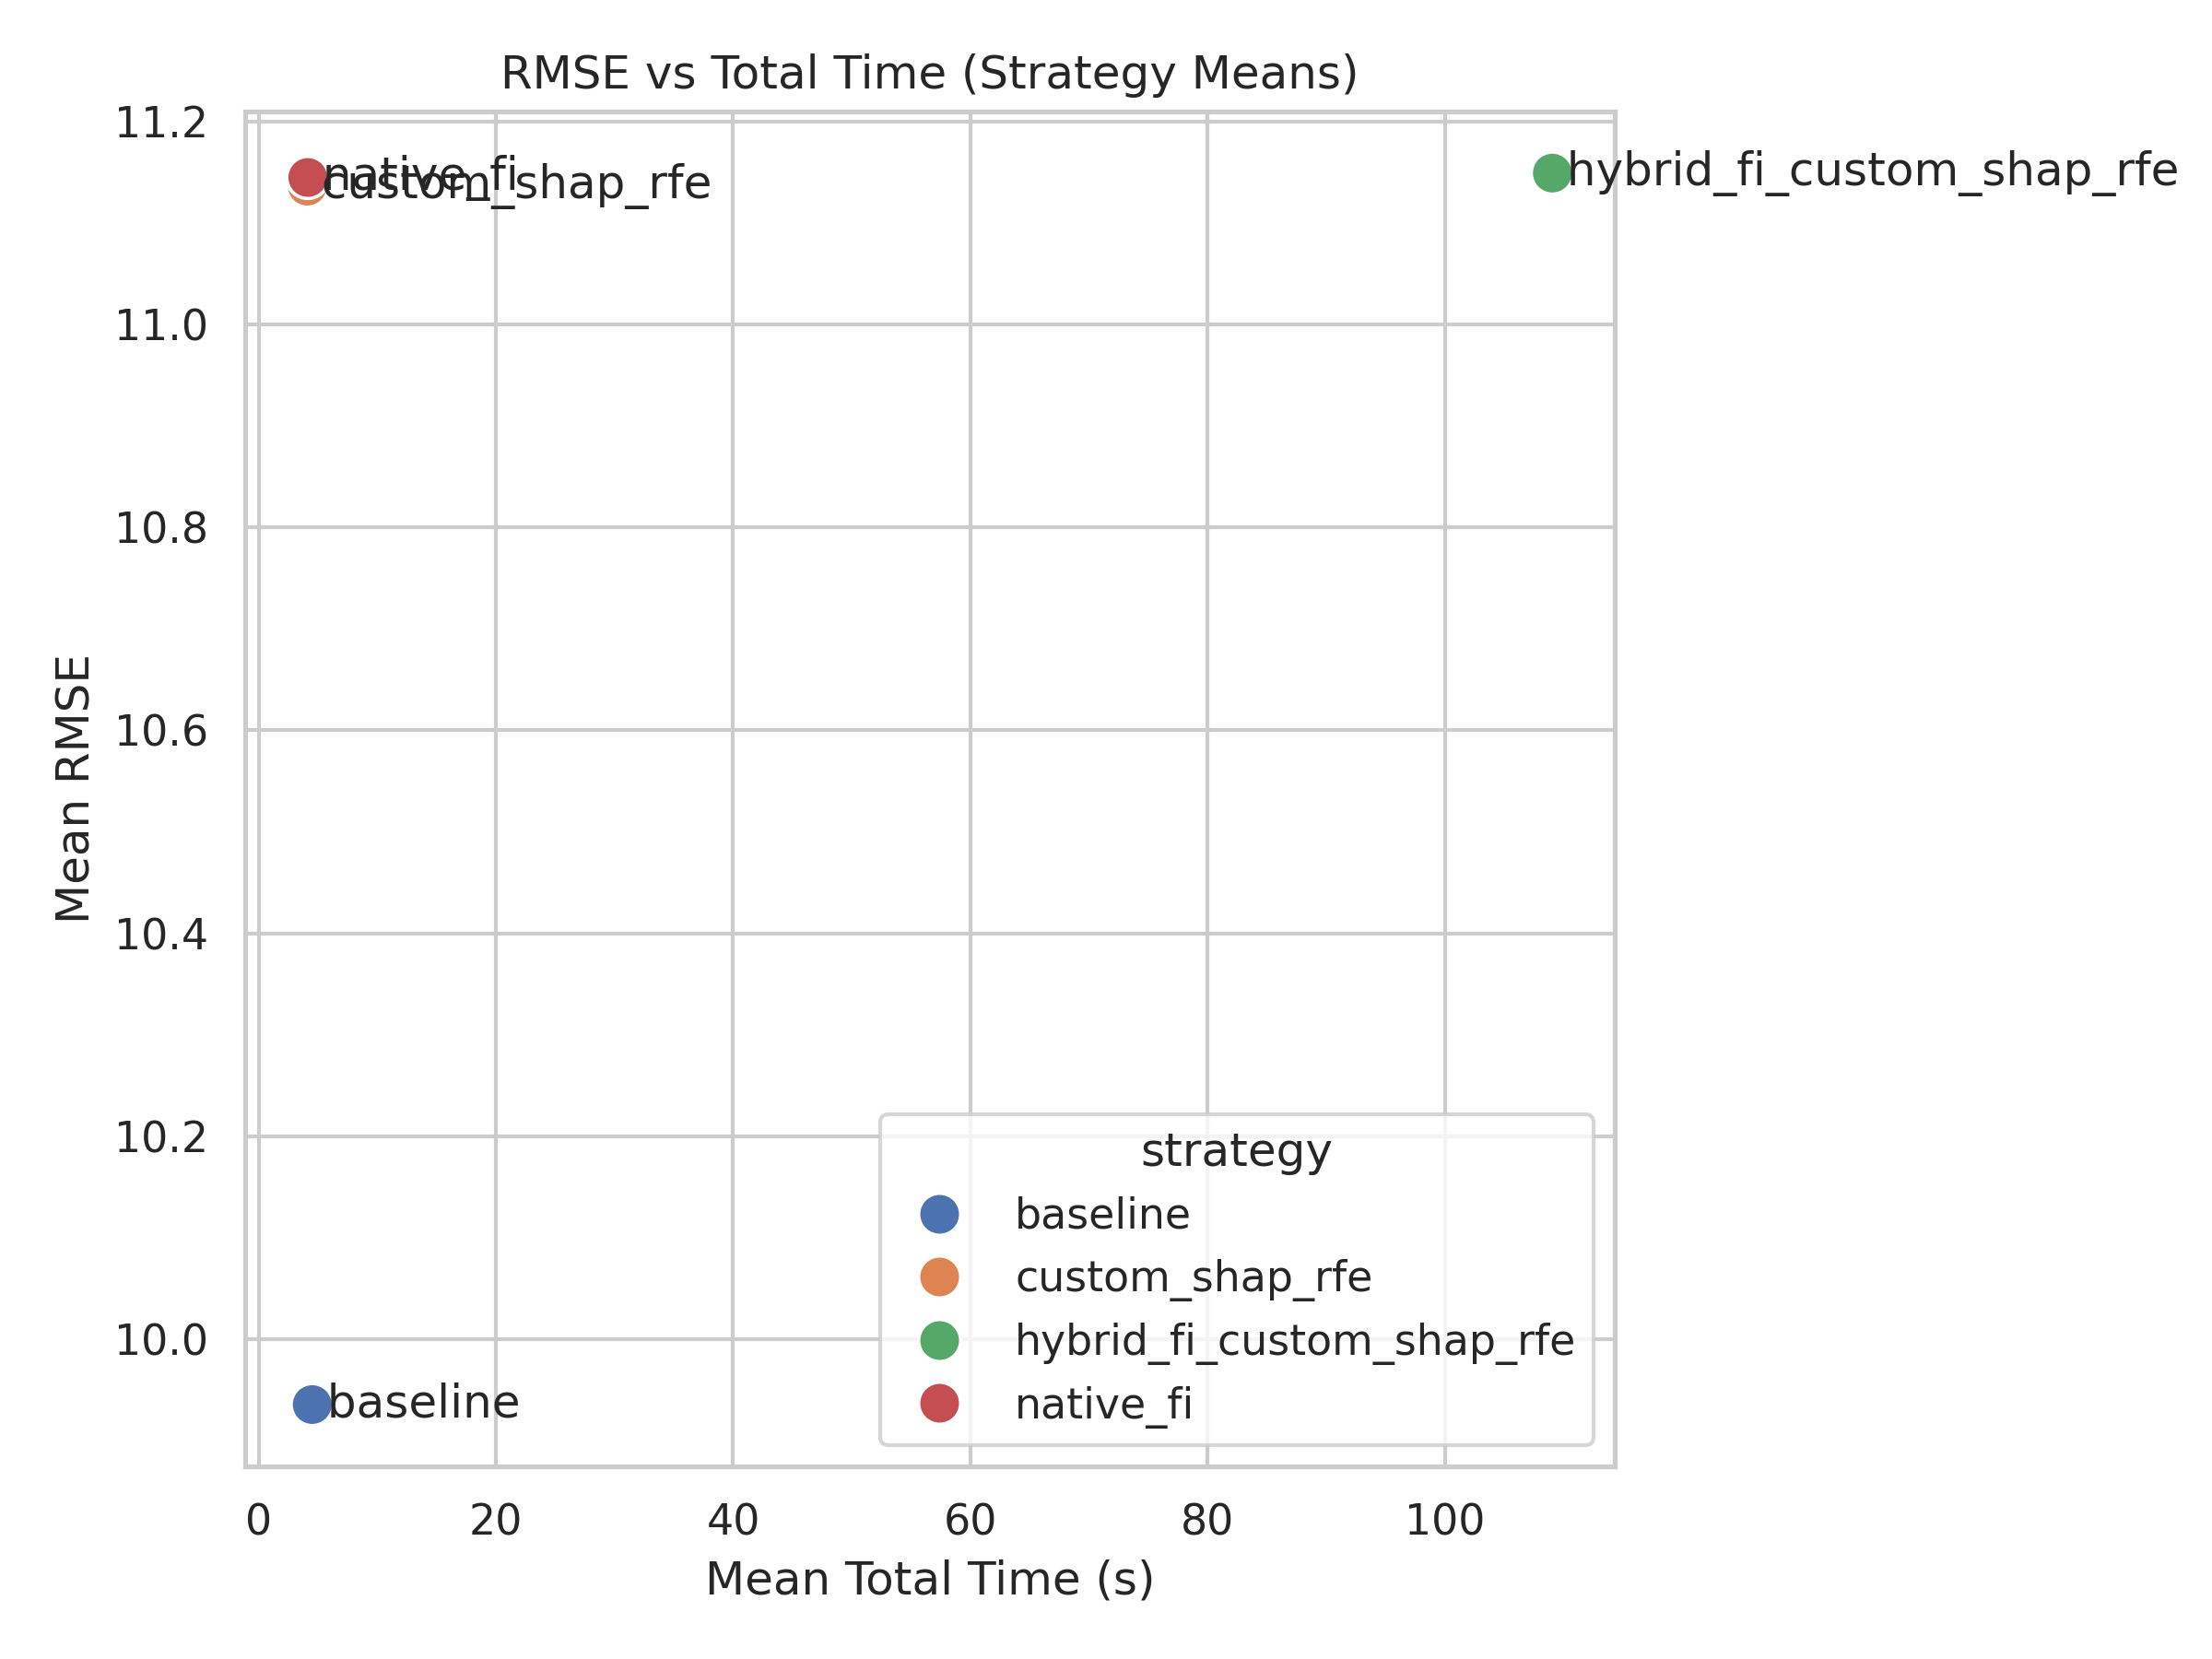
\includegraphics[width=0.48\textwidth]{../runs/exp2_run12/figures/exp2_rmse_vs_time_tradeoff.png}
    \caption{Superconductor deep-dive: RMSE by retention level (left) and RMSE vs. total time trade-off (right).}
    \label{fig:stage2_super}
\end{figure}

\subsection{Allstate Claims Dataset}

Table~\ref{tab:stage2_allstate} presents corresponding results for the Allstate dataset.

\begin{table}[h]
\centering
\caption{Allstate Claims results: RMSE and total time by strategy and retention level.}
\label{tab:stage2_allstate}
\begin{tabular}{llrr}
\toprule
\textbf{Strategy} & \textbf{k} & \textbf{RMSE} & \textbf{Time (s)} \\
\midrule
native\_fi & 0.05 & 2198.79 & 7.86 \\
custom\_shap\_rfe & 0.05 & 2277.81 & 7.52 \\
hybrid & 0.05 & 2224.63 & 129.69 \\
\midrule
native\_fi & 0.10 & 2062.39 & 7.96 \\
custom\_shap\_rfe & 0.10 & 2088.88 & 7.94 \\
hybrid & 0.10 & 2016.12 & 135.12 \\
\midrule
native\_fi & 0.25 & 1929.38 & 8.31 \\
custom\_shap\_rfe & 0.25 & 1925.70 & 8.50 \\
hybrid & 0.25 & 1932.26 & 152.25 \\
\midrule
native\_fi & 0.50 & 1912.92 & 8.93 \\
custom\_shap\_rfe & 0.50 & 1913.03 & 9.31 \\
hybrid & 0.50 & 1913.72 & 180.42 \\
\midrule
baseline & 1.00 & 1913.12 & 9.94 \\
\bottomrule
\end{tabular}
\end{table}

On Allstate, patterns are similar to Superconductor:

\textbf{Feature selection matches baseline}: At $k=0.50$, native\_fi achieves RMSE 1912.92, essentially identical to the baseline (1913.12). Selection provides no meaningful improvement.

\textbf{SHAP-RFE occasionally wins}: At $k=0.25$, custom\_shap\_rfe achieves the best RMSE (1925.70), marginally better than native\_fi (1929.38). This is consistent with hypothesis H2---small gains at intermediate retention.

\textbf{Hybrid underperforms and costs more}: At $k=0.50$, hybrid produces the worst RMSE (1913.72) among selection methods while requiring 20x more time than native\_fi.

Figure~\ref{fig:stage2_allstate} shows the trade-off visualization.

\begin{figure}[h]
    \centering
    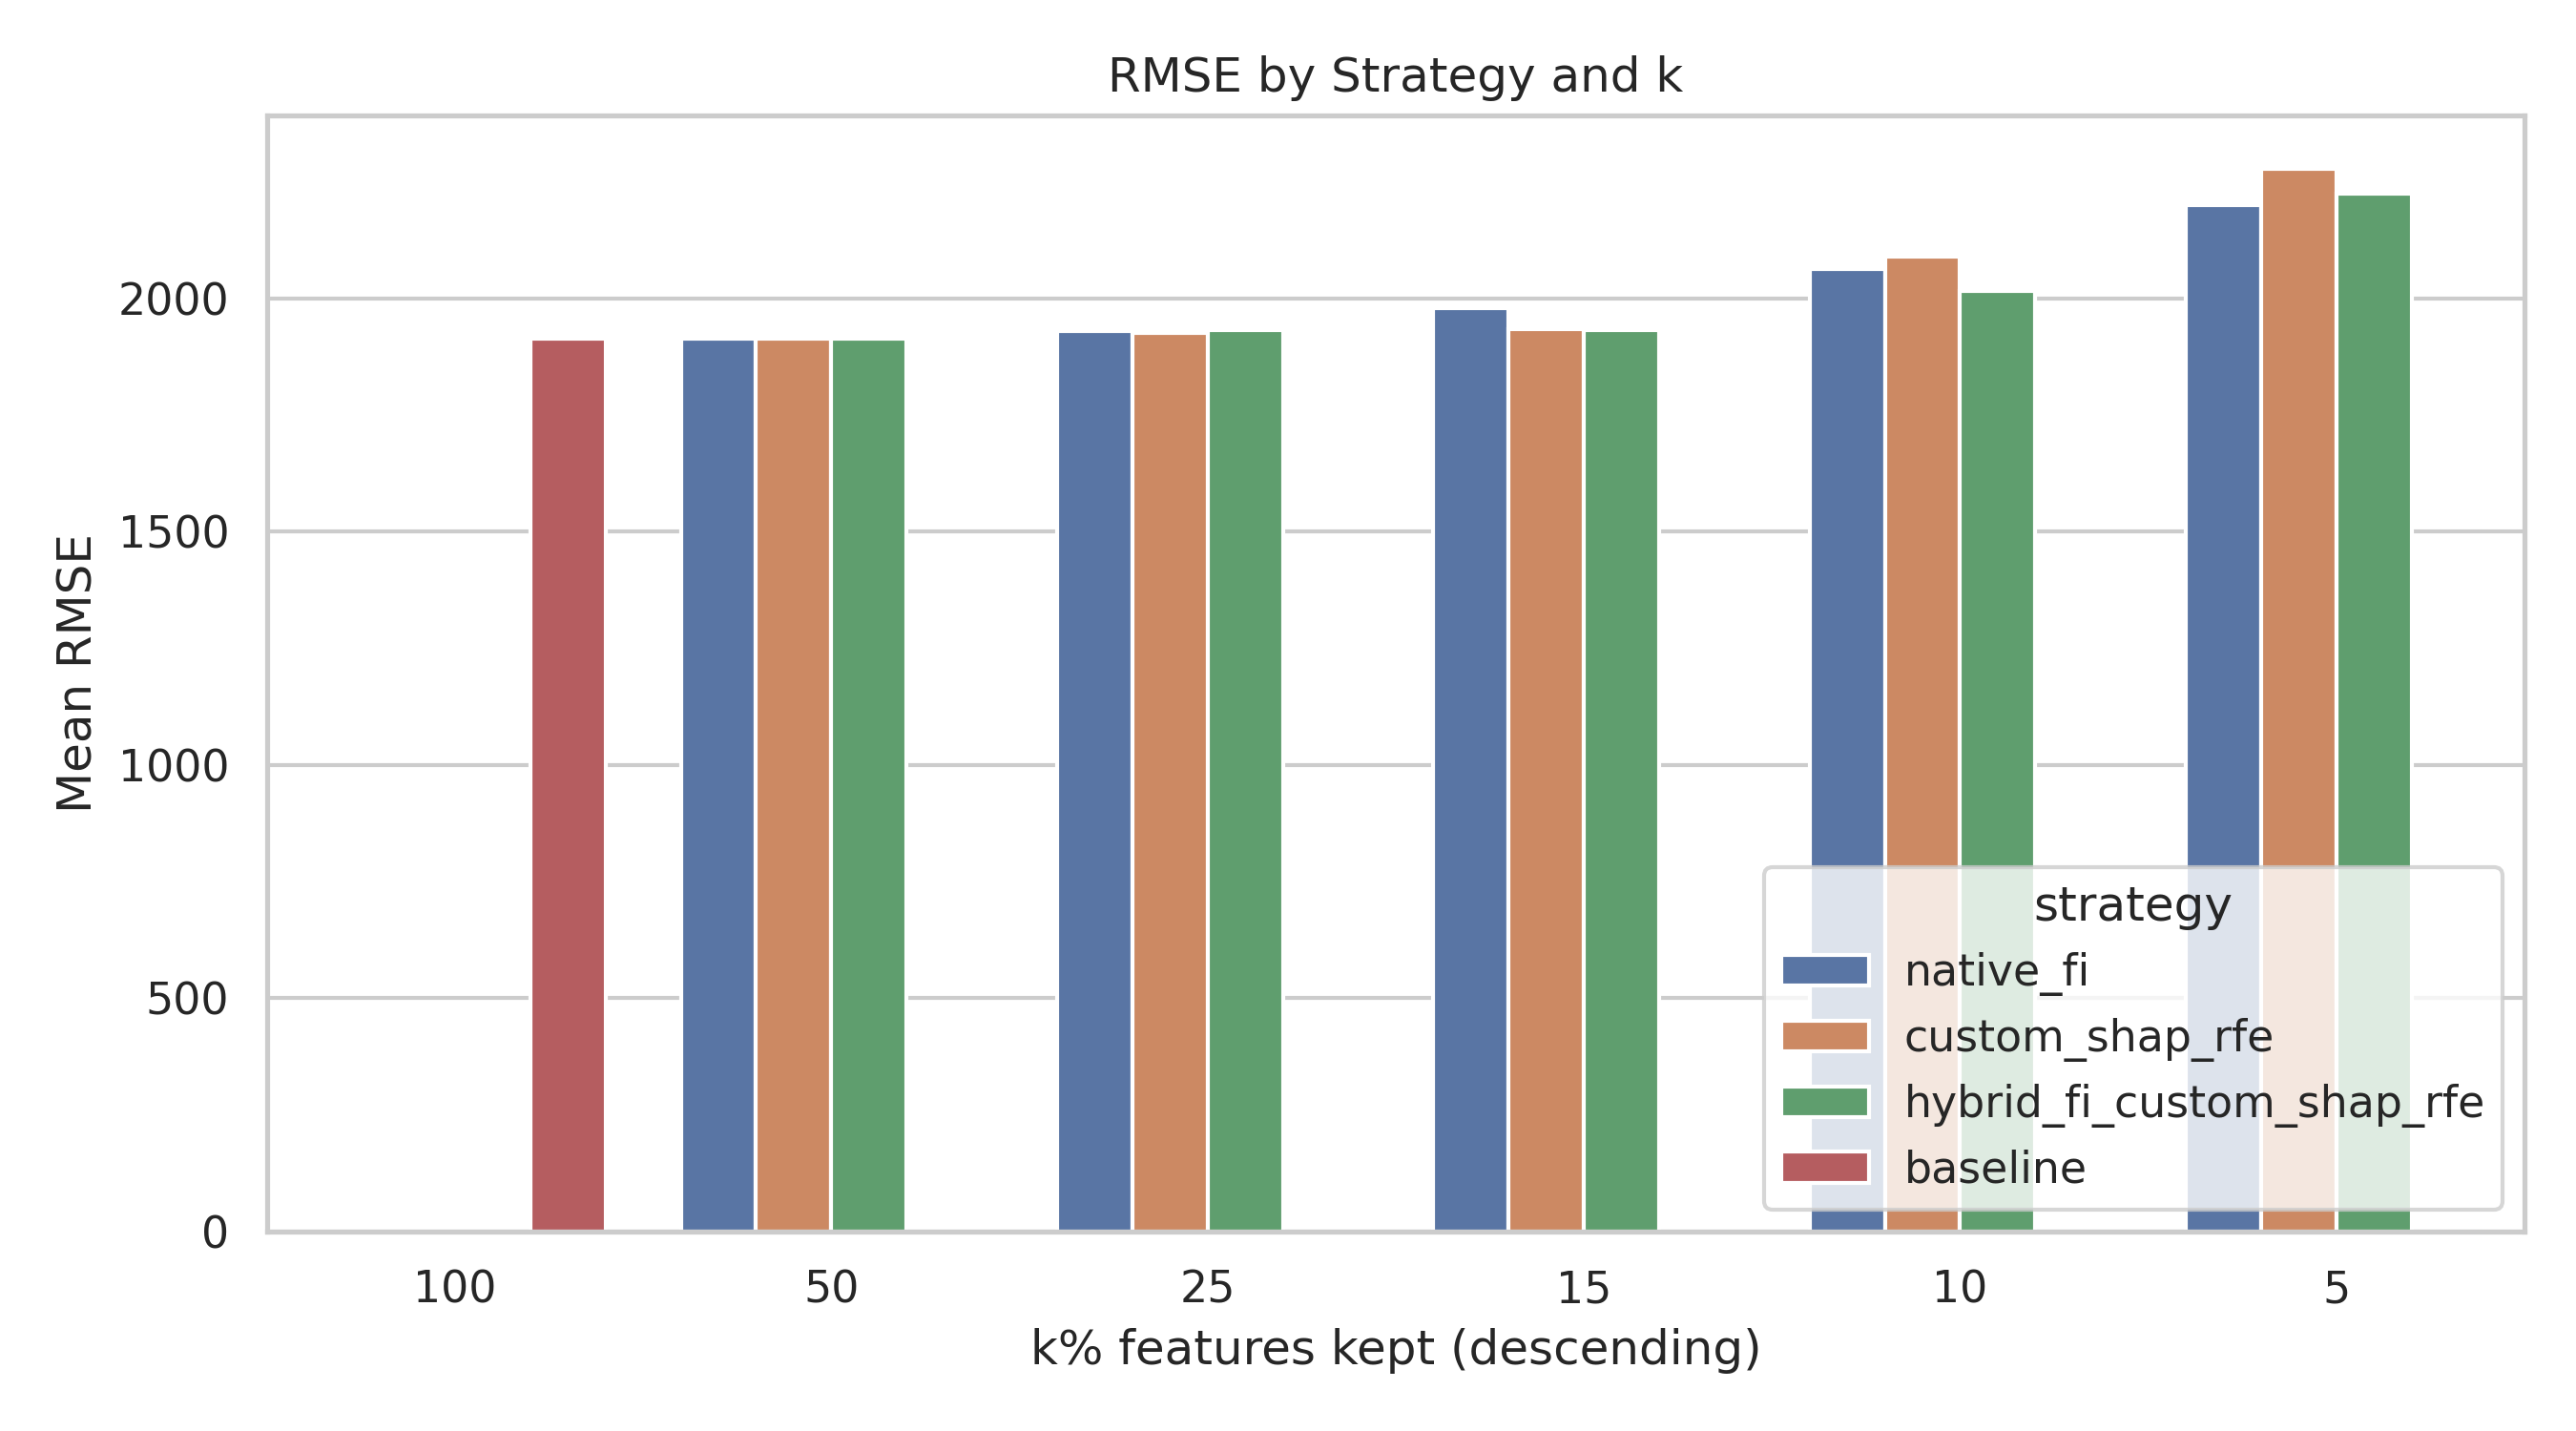
\includegraphics[width=0.48\textwidth]{../runs/exp3_run01/figures/exp3_rmse_by_strategy_k.png}
    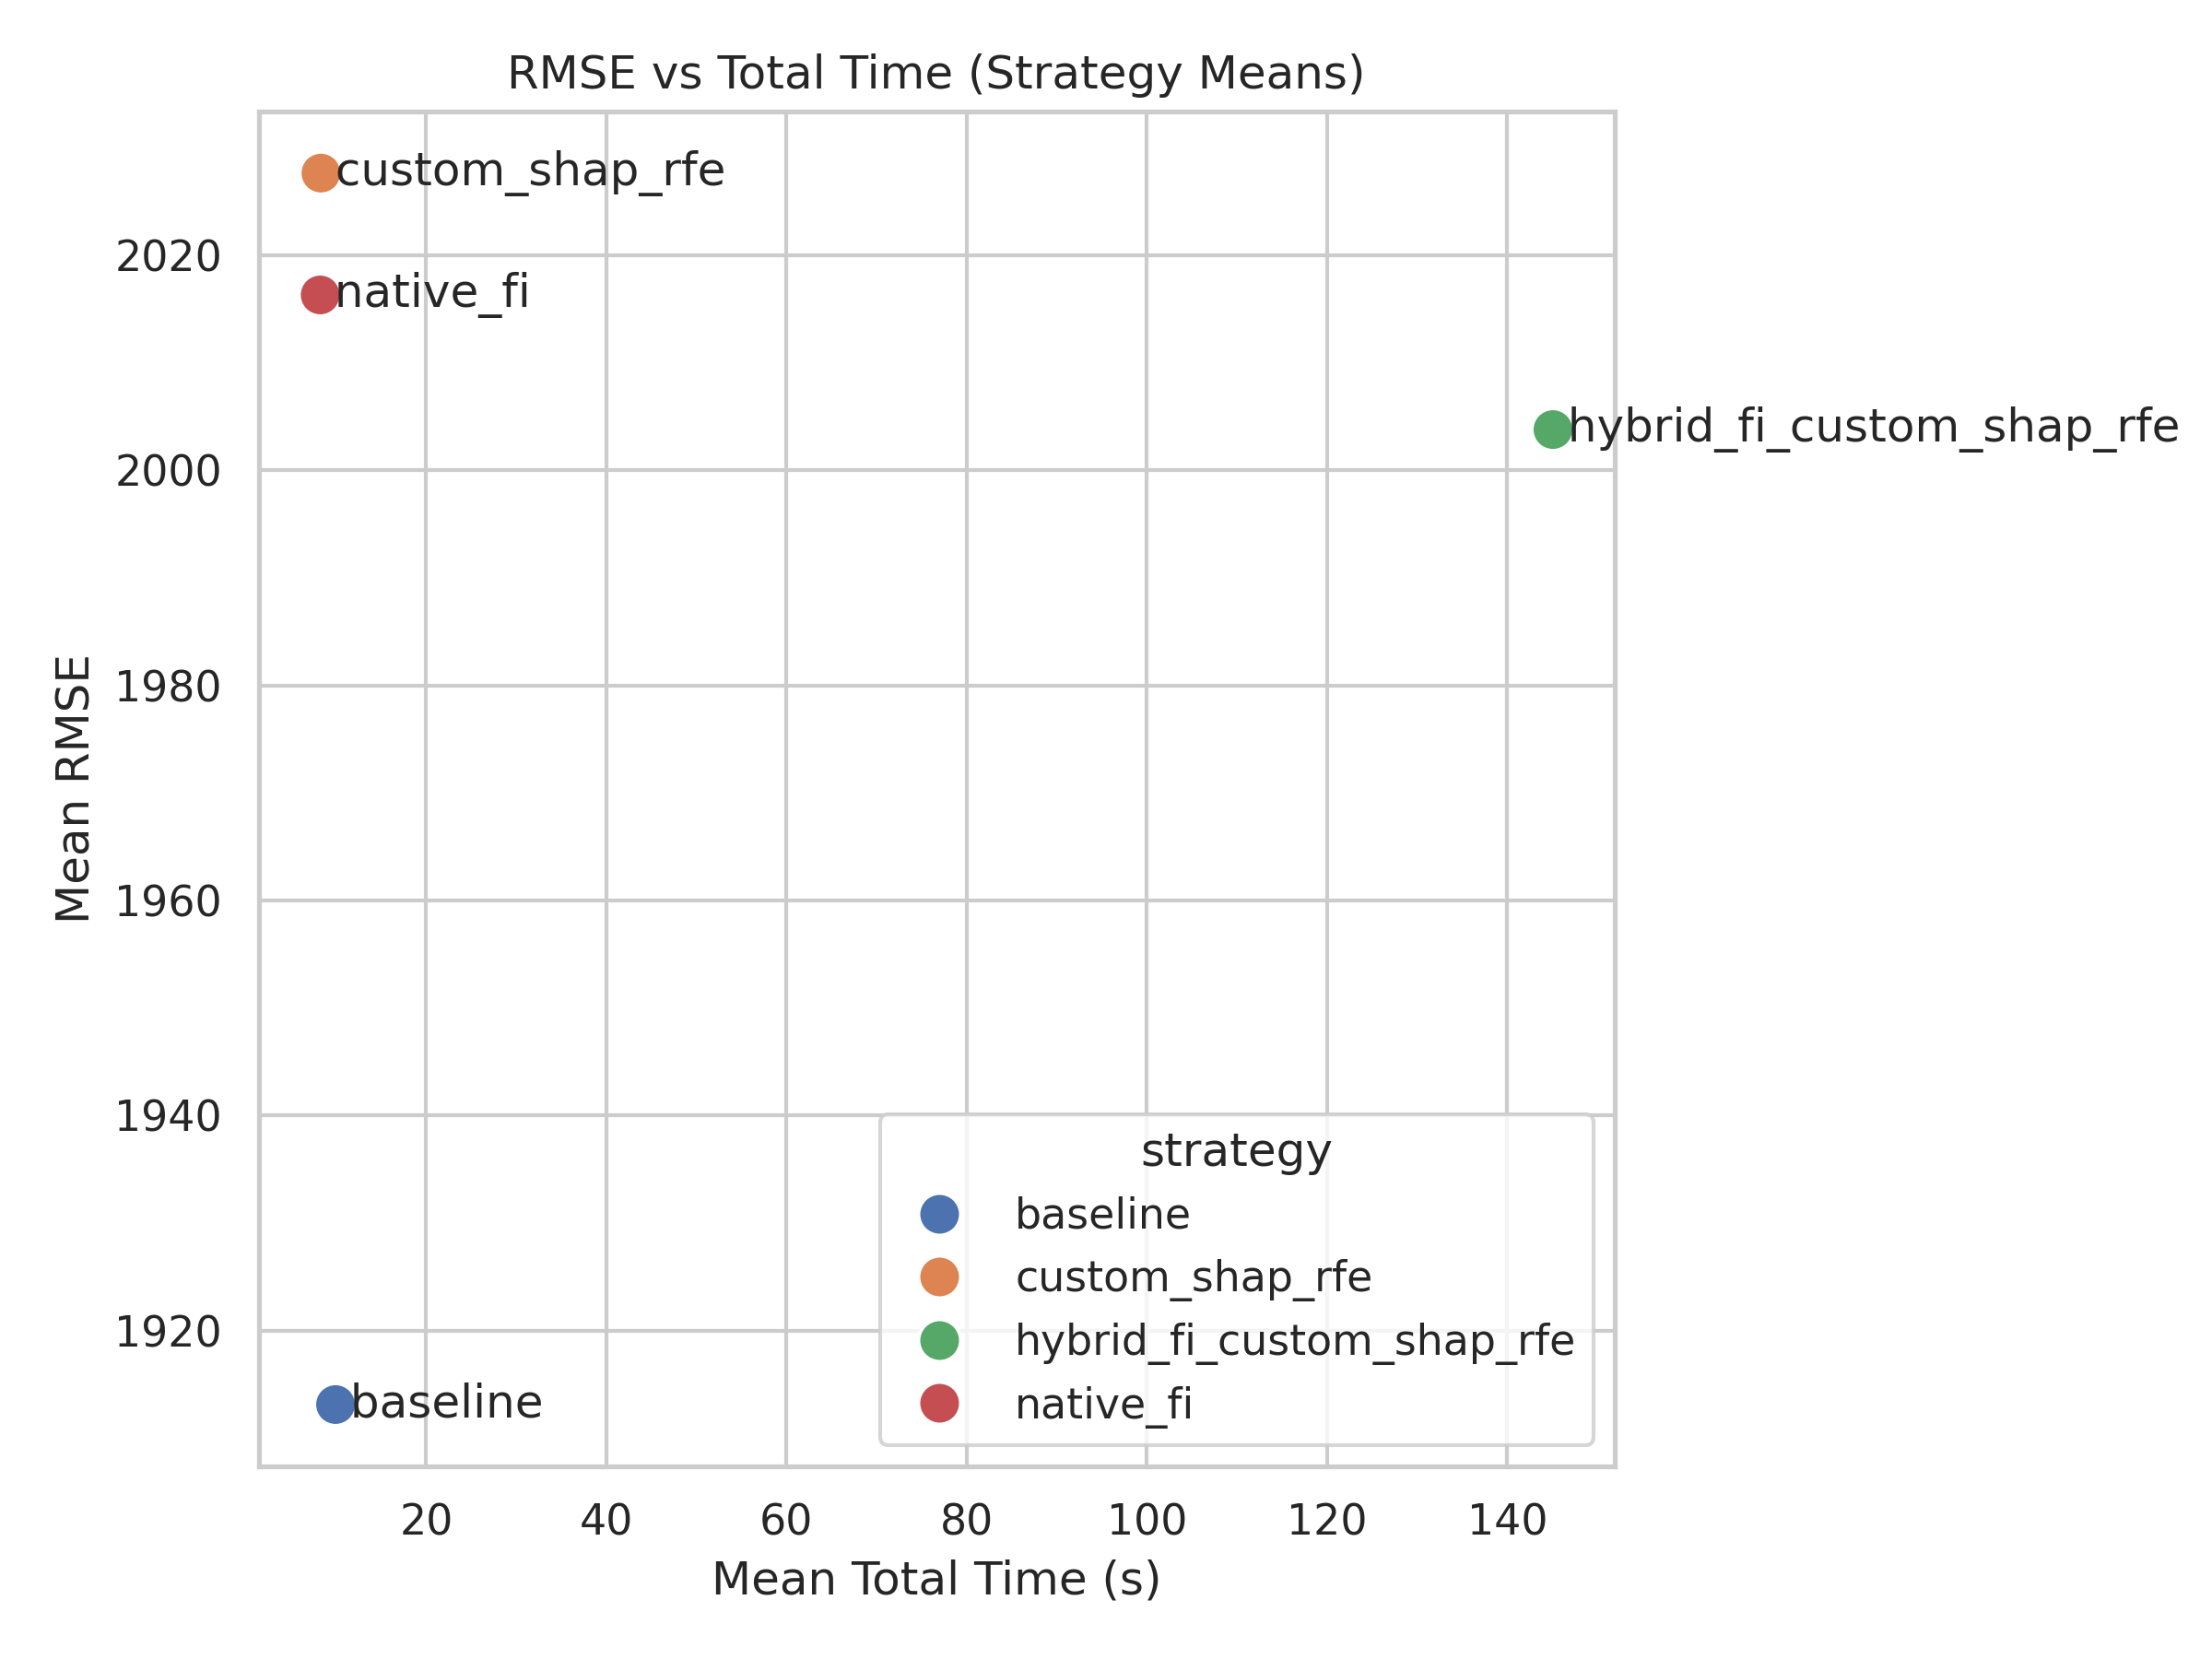
\includegraphics[width=0.48\textwidth]{../runs/exp3_run01/figures/exp3_rmse_vs_time_tradeoff.png}
    \caption{Allstate Claims deep-dive: RMSE by retention level (left) and RMSE vs. total time trade-off (right).}
    \label{fig:stage2_allstate}
\end{figure}

\subsection{Stability in Stage 2}

Figure~\ref{fig:stage2_stability} shows selection stability across retention levels for both datasets.

\begin{figure}[h]
    \centering
    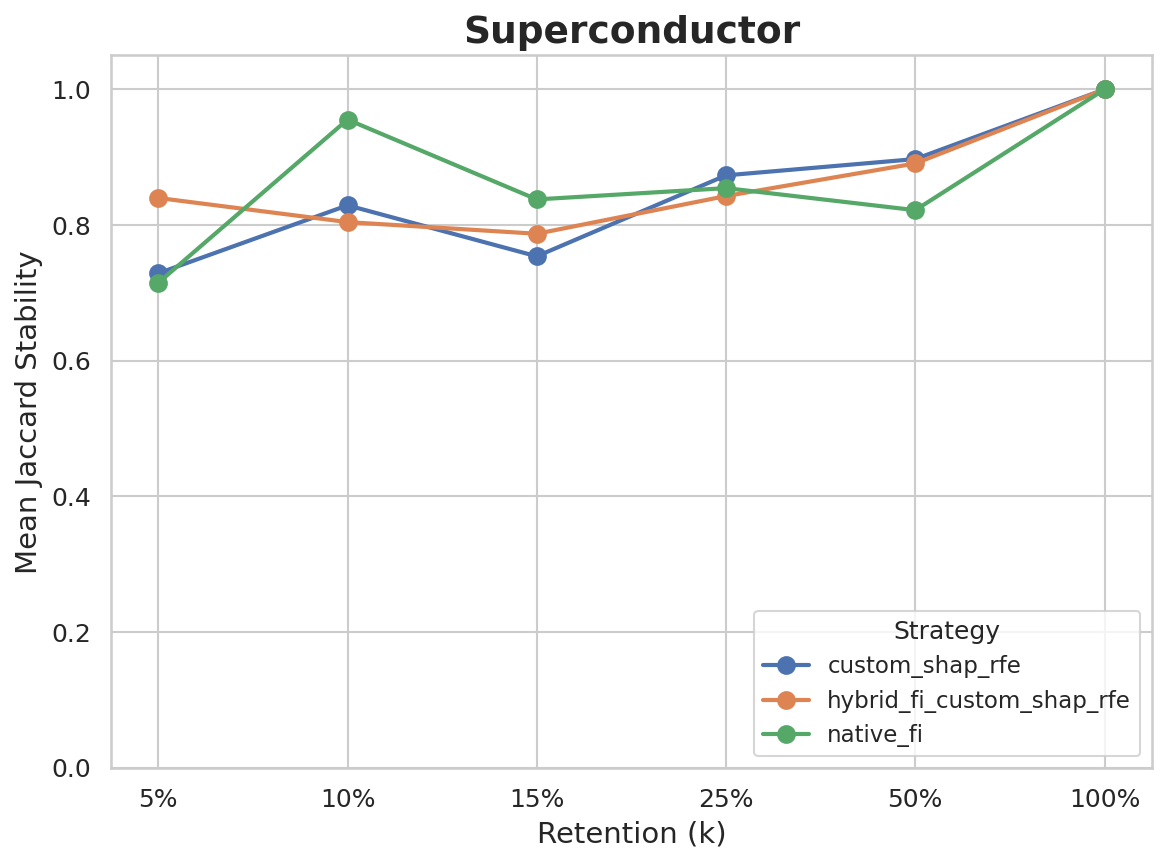
\includegraphics[width=0.48\textwidth]{../runs/exp2_run12/figures/exp2_stability_by_strategy_k.png}
    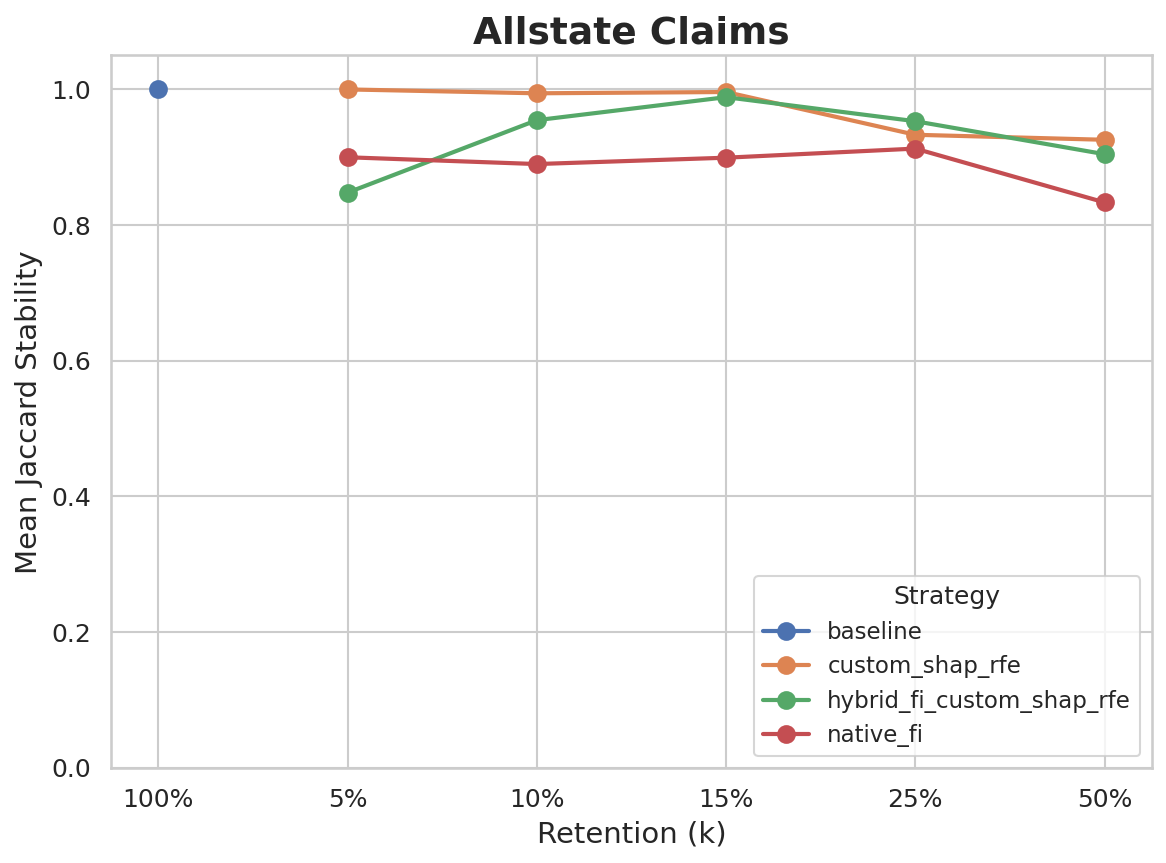
\includegraphics[width=0.48\textwidth]{../runs/exp3_run01/figures/exp3_stability_by_strategy_k.png}
    \caption{Selection stability in Stage~2: Superconductor (left) and Allstate (right).}
    \label{fig:stage2_stability}
\end{figure}

Stability follows expected patterns: lower at aggressive retention ($k=0.05$) and higher as more features are retained. Custom\_shap\_rfe shows notably high stability on Allstate at low $k$, suggesting that SHAP rankings are relatively consistent despite the model's stochasticity. The hybrid strategy's stability is comparable to simpler methods, providing no stability advantage to justify its cost.

\section{Synthesis and Hypothesis Evaluation}

The combined evidence from both stages supports the following conclusions:

\textbf{H1 (Competitive but non-dominant)}: \textit{Supported}. SHAP-based selection wins in 2 of 12 Stage~1 configurations, both with XGBoost. It is competitive but not dominant.

\textbf{H2 (Marginal gains at intermediate retention)}: \textit{Partially supported}. Small RMSE improvements appear at $k=0.25$ to $k=0.50$ in select cases (Allstate XGBoost with SHAP in Stage~1; custom\_shap\_rfe at $k=0.25$ in Stage~2 Allstate). However, these gains are minimal ($<1\%$ relative improvement).

\textbf{H3 (Substantial computational overhead)}: \textit{Supported}. The hybrid strategy consistently requires 20-30x more time than native\_fi with no systematic accuracy benefit. Even custom\_shap\_rfe, while faster, offers negligible advantage over native importance.

\textbf{H4 (Reduced stability at low retention)}: \textit{Partially supported}. Stability does decrease at low $k$ for all methods, but SHAP-based methods do not show dramatically worse stability than alternatives. In some cases (custom\_shap\_rfe on Allstate), SHAP stability is high.

\section{Threats to Validity}

Several limitations affect the generalizability of these findings:

\textbf{Dataset selection}: Four datasets cannot represent all tabular regression problems. Different domains or data characteristics might yield different conclusions.

\textbf{Hyperparameter choices}: Models were run with default or lightly-tuned hyperparameters. Joint optimization of feature selection and model hyperparameters might change relative rankings.

\textbf{Implementation details}: The custom SHAP-RFE and hybrid strategies are specific implementations. Alternative designs (e.g., different step sizes, pruning thresholds) might perform differently.

\textbf{Synthetic backfilling}: In Stage~1 data harmonization, some missing rows were interpolated. This caveat is acknowledged but does not affect the cleaner Stage~2 comparisons.

\section{Chapter Summary}

The experimental results demonstrate that SHAP-based feature selection, while theoretically principled and occasionally achieving the best RMSE, does not provide consistent practical advantages over simpler alternatives. Mutual Information and native tree importance frequently match or exceed SHAP performance at lower computational cost. The hybrid strategy, designed to combine the best of both worlds, instead combines computational expense with marginal performance. These findings suggest that practitioners should default to simpler methods and reserve SHAP-based selection for cases where its value has been demonstrated on the specific task at hand.

\chapter{Conclusions and Future Work}

This final chapter synthesizes the findings from the experimental investigation, draws practical conclusions for feature selection in regression workflows, and identifies directions for extending this work.

\section{Summary of Findings}

This thesis evaluated SHAP-based feature selection for tabular regression through a two-stage experimental protocol. The first stage screened four selection strategies across four datasets and three model families, while the second stage performed a focused analysis of SHAP-intensive methods using XGBoost on two selected datasets.

The central finding is that SHAP-based feature selection, despite its theoretical elegance and growing popularity in the interpretability literature, does not provide consistent practical advantages over simpler alternatives in the regression settings studied here. The evidence can be summarized along three dimensions:

\textbf{Predictive effectiveness}: SHAP achieved the best RMSE in only 2 of 12 dataset-model configurations in Stage~1, both with XGBoost. In Stage~2's focused comparison, custom SHAP recursive elimination occasionally outperformed native importance at intermediate retention levels, but gains were marginal---typically less than 1\% relative improvement. In many configurations, the full-feature baseline matched or exceeded all selection methods.

\textbf{Computational cost}: The hybrid strategy, which combines initial pruning with SHAP-guided elimination, consistently required 20-30 times more computation than simpler alternatives without delivering corresponding accuracy gains. Even straightforward SHAP ranking incurs overhead compared to native importance, particularly for bagging ensembles where TreeExplainer is less efficient.

\textbf{Selection stability}: SHAP-based methods showed somewhat lower stability at aggressive retention levels ($k=0.25$) in Stage~1. However, this pattern was not dramatic, and in Stage~2 the custom SHAP-RFE strategy demonstrated high stability on some configurations. Stability concerns do not strongly differentiate SHAP from alternatives.

\section{Interpretation}

These results do not suggest that SHAP is without value---it remains a powerful tool for model explanation and generating interpretable feature attributions. However, the evidence does not support treating SHAP importance as a superior feature selection criterion in general regression practice.

The lack of consistent SHAP advantage may reflect several factors:

\begin{itemize}
    \item \textbf{Redundancy with native importance}: For tree-based models, SHAP values and native importance scores often correlate strongly. Both capture similar information about feature contribution, so the additional computation for SHAP may not surface truly different rankings.

    \item \textbf{Model robustness}: Modern gradient boosting and ensemble methods are reasonably robust to irrelevant features. When models can internally down-weight uninformative variables, explicit selection provides diminishing returns.

    \item \textbf{Dataset characteristics}: The datasets used, while diverse, may not exhibit the specific conditions where SHAP-based selection would shine---for example, settings with many features of similar importance where fine-grained ranking matters.
\end{itemize}

\section{Practical Recommendations}

Based on the experimental evidence, the following guidelines are offered for practitioners approaching feature selection in tabular regression:

\begin{enumerate}
    \item \textbf{Start simple}: Begin with a full-feature baseline using a regularized or tree-based model. Many datasets do not benefit from explicit selection, and this baseline provides a reference point.

    \item \textbf{Use low-cost methods first}: If selection is desired, mutual information or native importance rankings provide competitive results at minimal computational cost. These should be the default choices for initial exploration.

    \item \textbf{Reserve SHAP for targeted use}: SHAP-based selection may be justified when (a) the practitioner has specific evidence that it improves performance on the task at hand, or (b) the primary goal is interpretability rather than raw accuracy, and SHAP attributions align better with domain understanding.

    \item \textbf{Avoid expensive hybrids without validation}: Hybrid strategies that combine multiple selection passes do not automatically outperform simpler methods. Their complexity and cost should be justified by demonstrated gains on representative validation data.

    \item \textbf{Consider the full trade-off}: Evaluation should always consider computational cost alongside accuracy. A method that achieves marginally lower RMSE but requires significantly more time may not be preferable in production or iterative development contexts.
\end{enumerate}

\section{Limitations}

This thesis has several limitations that constrain the generalizability of conclusions:

\begin{itemize}
    \item \textbf{Scope}: Four datasets and three model families cannot represent the full diversity of regression problems. Results may differ on time-series data, extremely high-dimensional settings, or domains with specific structure.

    \item \textbf{Hyperparameters}: Models were run with default or lightly-tuned configurations. Joint optimization of feature selection and model hyperparameters might reveal different patterns.

    \item \textbf{Strategy implementations}: The custom SHAP-RFE and hybrid approaches are specific implementations. Alternative designs might perform better or worse.

    \item \textbf{Metrics}: The study focused on RMSE, stability, and runtime. Other considerations---interpretability of selected features, downstream deployment constraints, or regulatory requirements---might favor different choices.
\end{itemize}

\section{Future Work}

Several directions could extend and refine the findings of this thesis:

\textbf{Broader dataset coverage}: Evaluating on additional domains (healthcare, finance, industrial sensors) would test whether the observed patterns generalize or are specific to the datasets studied here.

\textbf{Alternative model architectures}: Extending the comparison to neural tabular models (e.g., TabNet, NODE) or other boosting implementations (LightGBM, CatBoost) would assess whether conclusions transfer across model families.

\textbf{Joint optimization}: Investigating nested hyperparameter tuning where feature selection parameters are optimized alongside model hyperparameters could reveal interactions that fixed-configuration studies miss.

\textbf{Cost-aware selection}: Developing adaptive strategies that trigger SHAP computation only when uncertainty about feature rankings is high might reduce overhead while preserving potential benefits.

\textbf{Alternative stability definitions}: Exploring consensus-based selection mechanisms that aggregate rankings across multiple model fits could improve robustness without the expense of full SHAP computation at each iteration.

\textbf{Interpretability-focused evaluation}: Extending evaluation to include human-centered metrics---how well selected features align with domain expert expectations, or how interpretable the resulting models are---would address dimensions beyond raw accuracy.

\section{Closing Remarks}

This thesis set out to answer a practical question: does SHAP-based feature selection justify its computational cost in tabular regression? The evidence suggests a measured answer: SHAP is a useful but expensive tool that provides at best marginal advantages over simpler alternatives in the settings studied. For practitioners working under computational or time constraints, simpler methods remain the pragmatic default. SHAP's value lies primarily in its explanatory power, not as a feature selection criterion. Future work may identify conditions where SHAP-based selection is more clearly advantageous, but until such conditions are characterized, a conservative approach is warranted.

\bibliographystyle{plain}
\bibliography{references}
\addcontentsline{toc}{chapter}{Bibliography}


\end{document}
